\documentclass[12pt,a4paper]{article}
\usepackage[utf8]{inputenc}
\usepackage[spanish]{babel}
\usepackage{geometry}
\usepackage{amsmath}
\usepackage{amssymb}
\usepackage{booktabs}
\usepackage{longtable}
\usepackage{graphicx}
\usepackage{enumitem}
\usepackage{float}
\usepackage{xcolor}
\usepackage{fancyhdr}
\usepackage{caption}
\usepackage[numbers]{natbib}
\usepackage[colorlinks=true,linkcolor=black,citecolor=blue,urlcolor=blue]{hyperref}

\geometry{margin=2.5cm}

\pagestyle{fancy}
\fancyhf{}
\fancyhead[L]{T6 – Rejillas + Desarenador + ABR-RAP + Humedal Vertical + Cloro + Lecho de Secado}
\fancyhead[R]{\thepage}

\setcounter{tocdepth}{2}

\begin{document}

\begin{titlepage}
\centering
\vspace*{2cm}

{\Huge\bfseries Memoria de Cálculo\par}
\vspace{1.5cm}

{\Large\itshape Dimensionamiento de:\par}
\vspace{0.5cm}

{\LARGE\bfseries T6 – Rejillas + Desarenador + ABR-RAP + Humedal Vertical + Cloro + Lecho de Secado\par}
\vspace{2cm}

{\large Caudal de diseño: 17.31 L/s\par}
{\large Número de líneas: 3\par}
\vfill
{\large\today\par}
\end{titlepage}

\tableofcontents

\listoffigures

\listoftables

\newpage
\section{Resumen del Proyecto}

Este documento presenta el dimensionamiento detallado del T6 – Rejillas + Desarenador + ABR-RAP + Humedal Vertical + Cloro + Lecho de Secado, disenado para tratar un caudal de 17.31 L/s distribuido en 3 lineas paralelas (5.77 L/s por linea).

\textbf{Caracteristicas del afluente:}
\begin{itemize}
    \item DBO$_5$: 243.1 mg/L
    \item DQO: 498.0 mg/L
    \item SST: 156.0 mg/L
    \item Coliformes fecales: 3e+03 NMP/100mL
    \item Temperatura: 25.6°C
\end{itemize}

\textbf{Secuencia de unidades del tren:} 
Canal de Desbaste con Rejillas $\rightarrow$ Desarenador de Flujo Horizontal $\rightarrow$ Reactor Anaerobio con Pantallas (ABR/RAP) $\rightarrow$ Humedal Artificial de Flujo Vertical (HAFV) $\rightarrow$ Sistema de Desinfeccion con Hipoclorito de Sodio $\rightarrow$ Lechos de Secado de Lodos

\newpage
\section{Dimensionamiento de Unidades}

\subsection{Canal de Desbaste con Rejillas}

\

Las rejillas constituyen la primera barrera de proteccion del sistema, reteniendo solidos gruesos como plasticos, ramas y papel que podrian danar equipos o causar obstrucciones en tuberias aguas abajo. El diseno hidraulico de esta unidad debe garantizar velocidades suficientes para arrastrar solidos sedimentables, pero no tan elevadas que dificulten el paso del agua a traves de las barras.

Segun los criterios establecidos por Metcalf y Eddy \cite{metcalf2014}, las velocidades de diseno en canales con rejillas deben mantenerse entre 0.40 y 0.60~m/s. Para este proyecto se adopta un valor intermedio de 0.50~m/s, lo cual resulta apropiado considerando el caudal de diseno. El tirante hidraulico se establece en 0.40~m, valor que permite una velocidad de flujo uniforme en la seccion del canal y evita la sedimentacion de solidos organicos antes de la rejilla, segun los criterios de Metcalf y Eddy \cite{metcalf2014}.

La perdida de carga en rejillas limpias se calcula mediante la formula de Kirschmer (1926), que relaciona la geometria de las barras con las caracteristicas del flujo. Los parametros que determinan esta perdida son: el espaciado entre barras ($b$), el espesor de las barras ($w$), la velocidad del flujo ($v$) y el angulo de inclinacion ($\theta$):

\begin{equation}
h_L = \beta \cdot \left(\frac{w}{b}\right)^{4/3} \cdot \frac{v^2}{2g} \cdot \sin\theta
\end{equation}
\captionequation{Perdida de carga en rejillas limpias - Formula de Kirschmer}

\textit{Donde:}
\begin{itemize}[noitemsep,leftmargin=2em]
    \item[$h_L$] = Perdida de carga en rejillas limpias (m)
    \item[$\beta$] = Factor de forma de la barra (2.42 para barras rectangulares)
    \item[$w$] = Espesor de la barra (10 mm)
    \item[$b$] = Espaciado entre barras (15 mm)
    \item[$v$] = Velocidad del flujo en el canal (m/s)
    \item[$g$] = Aceleracion de la gravedad (9,81 m/s\textsuperscript{2})
    \item[$\theta$] = Angulo de inclinacion de las barras (60\textdegree)
\end{itemize}

\begin{table}[H]
\centering
\caption{Parametros de diseno -- Rejillas}
\begin{tabular}{llcc}
\toprule
Parametro & Descripcion & Valor adoptado & Fuente \\
\midrule
Velocidad en canal & Velocidad de paso & 0.50 m/s & Metcalf y Eddy \\
Tirante hidraulico & Altura de agua en canal & 0.40 m & Criterio tecnico \\
Angulo de rejilla & Inclinacion barras & 60\textdegree & Practica comun \\
Espaciado entre barras & Abertura libre & 15 mm & OPS/CEPIS \\
Espesor de barras & Seccion barra & 10 mm & Constructivo \\
Factor de forma & Barras rectangulares & 2.42 & Kirschmer \\
\bottomrule
\end{tabular}
\end{table}

El caudal de diseno por linea es 5.8 L/s. La seccion transversal del canal se determina aplicando la ecuacion de continuidad:

\begin{equation}
A_{{canal}} = \frac{Q}{v} = \frac{0.00577}{0.50} = 0.01154 \text{ m}^2
\end{equation}

\textit{Donde:}
\begin{itemize}[noitemsep,leftmargin=2em]
    \item[$A_{{canal}}$] = Seccion transversal del canal (m\textsuperscript{2})
    \item[$Q$] = Caudal de diseno por linea (0.00577 m\textsuperscript{3}/s)
    \item[$v$] = Velocidad de diseno adoptada (0.50 m/s)
\end{itemize}

Despejando el ancho del canal de la ecuacion $A = b \times h$, con $h = 0.40$ m:

\begin{equation}
b = \frac{A_{{canal}}}{h} = \frac{0.01154}{0.40} = 0.029 \text{ m}
\end{equation}

\textit{Donde:}
\begin{itemize}[noitemsep,leftmargin=2em]
    \item[$b$] = Ancho teorico del canal (m)
    \item[$A_{{canal}}$] = Seccion transversal del canal (0.01154 m\textsuperscript{2})
    \item[$h$] = Tirante hidraulico (0.40 m)
\end{itemize}

Este ancho teorico de 0.029 m es inferior al minimo constructivo practico. Se adopta un ancho de 0.60 m como dimension minima constructiva segun criterios de OPS/CEPIS \cite{ops2005} y SENAGUA \cite{senagua2012}, que establecen un ancho minimo de 0.60 m para permitir la operacion adecuada, el acceso para limpieza y la aplicacion de herramientas de mantenimiento. Verificando la velocidad real con este ancho:

\begin{equation}
v_{{real}} = \frac{Q}{A_{{real}}} = \frac{0.00577}{0.60 \times 0.40} = 0.024 \text{ m/s}
\end{equation}

\textit{Donde:}
\begin{itemize}[noitemsep,leftmargin=2em]
    \item[$v_{{real}}$] = Velocidad real verificada con ancho constructivo (m/s)
    \item[$Q$] = Caudal de diseno (0.00577 m\textsuperscript{3}/s)
    \item[$A_{{real}}$] = Seccion real con ancho constructivo adoptado (0.60 $\times$ 0.40 m\textsuperscript{2})
\end{itemize}

La velocidad real de 0.024 m/s es el resultado de adoptar el ancho minimo constructivo. La perdida de carga calculada con esta velocidad real resulta $h_L = 0.0036$ cm, menor al umbral de 15 cm que Metcalf y Eddy \cite{metcalf2014} indican como referencia para sistemas de limpieza mecanica.

La longitud de 2.0 m y el ancho de 0.60 m responden a criterios constructivos y operativos. El ancho de 0.60 m es la dimension minima constructiva segun OPS/CEPIS \cite{ops2005} y SENAGUA \cite{senagua2012}, que permite la operacion adecuada de la rejilla, el acceso para limpieza y la aplicacion de herramientas de mantenimiento. La longitud contempla el espacio de la rejilla propiamente dicha mas las zonas de transicion necesarias para la operacion.





\subsubsection{Verificacion}

\textbf{Verificacion para Caudal Maximo Horario}

Se verifica el comportamiento hidraulico para el caudal maximo horario, aplicando un factor de pico tipico de 2.8 sobre el caudal medio:

\begin{equation}
Q_{{max}} = 2.8 \times Q_{{medio}} = 2.8 \times 5.8 = 16.0 \text{ L/s}
\end{equation}

A caudal maximo, la velocidad horizontal resulta:

\begin{equation}
v_{{max}} = \frac{Q_{{max}}}{A_{{real}}} = \frac{15.983/1000}{0.60 \times 0.40} = 0.067 \text{ m/s}
\end{equation}

\textbf{Criterios de verificacion de velocidad} (segun Metcalf y Eddy \cite{metcalf2014}):

La velocidad calculada $v_{{max}} = 0.067$~m/s se evalua segun:

\begin{equation}
\text{Estado} = \begin{cases}
    \text{OPTIMO} & \text{si } v_{{max}} \leq 1.5 \text{ m/s} \quad \text{(sin riesgo)} \\
    \text{ACEPTABLE} & \text{si } 1.5 < v_{{max}} \leq 2.0 \text{ m/s} \quad \text{(monitoreo)} \\
    \text{NO ADMISIBLE} & \text{si } v_{{max}} > 2.0 \text{ m/s} \quad \text{(dano seguro)}
\end{cases}
\end{equation}
\captionequation{Criterios de verificacion de velocidad en rejillas}

Con la velocidad calculada $v_{{max}} = 0.067$~m/s, la unidad se clasifica como \textbf{OPTIMO}. En terminos de cumplimiento, la verificacion de velocidad \textbf{CUMPLE} porque es menor que el limite recomendado de 1.5~m/s para operacion segura.

Respecto a la perdida de carga, el valor maximo calculado es 0.0276~cm. Por tanto, la verificacion de perdida de carga \textbf{CUMPLE}, ya que es menor que el umbral de 15~cm para limpieza manual aceptable.

\subsubsection{Resultados}

\begingroup
\small
\begin{longtable}{lccc}
\caption{Verificacion de criterios de diseno - Rejillas}\\
\toprule
Parametro & Valor calculado & Criterio & Estado \\
\midrule
\endfirsthead
\caption[]{Verificacion de criterios de diseno - Rejillas (continuación)}\\
\toprule
Parametro & Valor calculado & Criterio & Estado \\
\midrule
\endhead
\midrule
\multicolumn{4}{r}{\textit{Continúa en la siguiente página}} \\
\endfoot
\bottomrule
\endlastfoot
Velocidad de diseno & 0.50 m/s & 0.40 -- 0.60 m/s & Cumple \\
Velocidad real & 0.024 m/s & Ancho minimo constructivo$^a$ & Aplicado \\
Perdida de carga (Qmax) & 0.0276 cm & $<$ 15 cm & Cumple \\
Ancho constructivo & 0.60 m & $\geq$ 0.30 m & Cumple \\
\multicolumn{4}{p{\textwidth}}{\small $^a$ Para caudales pequenos (5.8 L/s) el ancho minimo constructivo (0.60 m) domina sobre el criterio de velocidad.} \\
\end{longtable}
\endgroup

\begin{figure}[H]
\centering
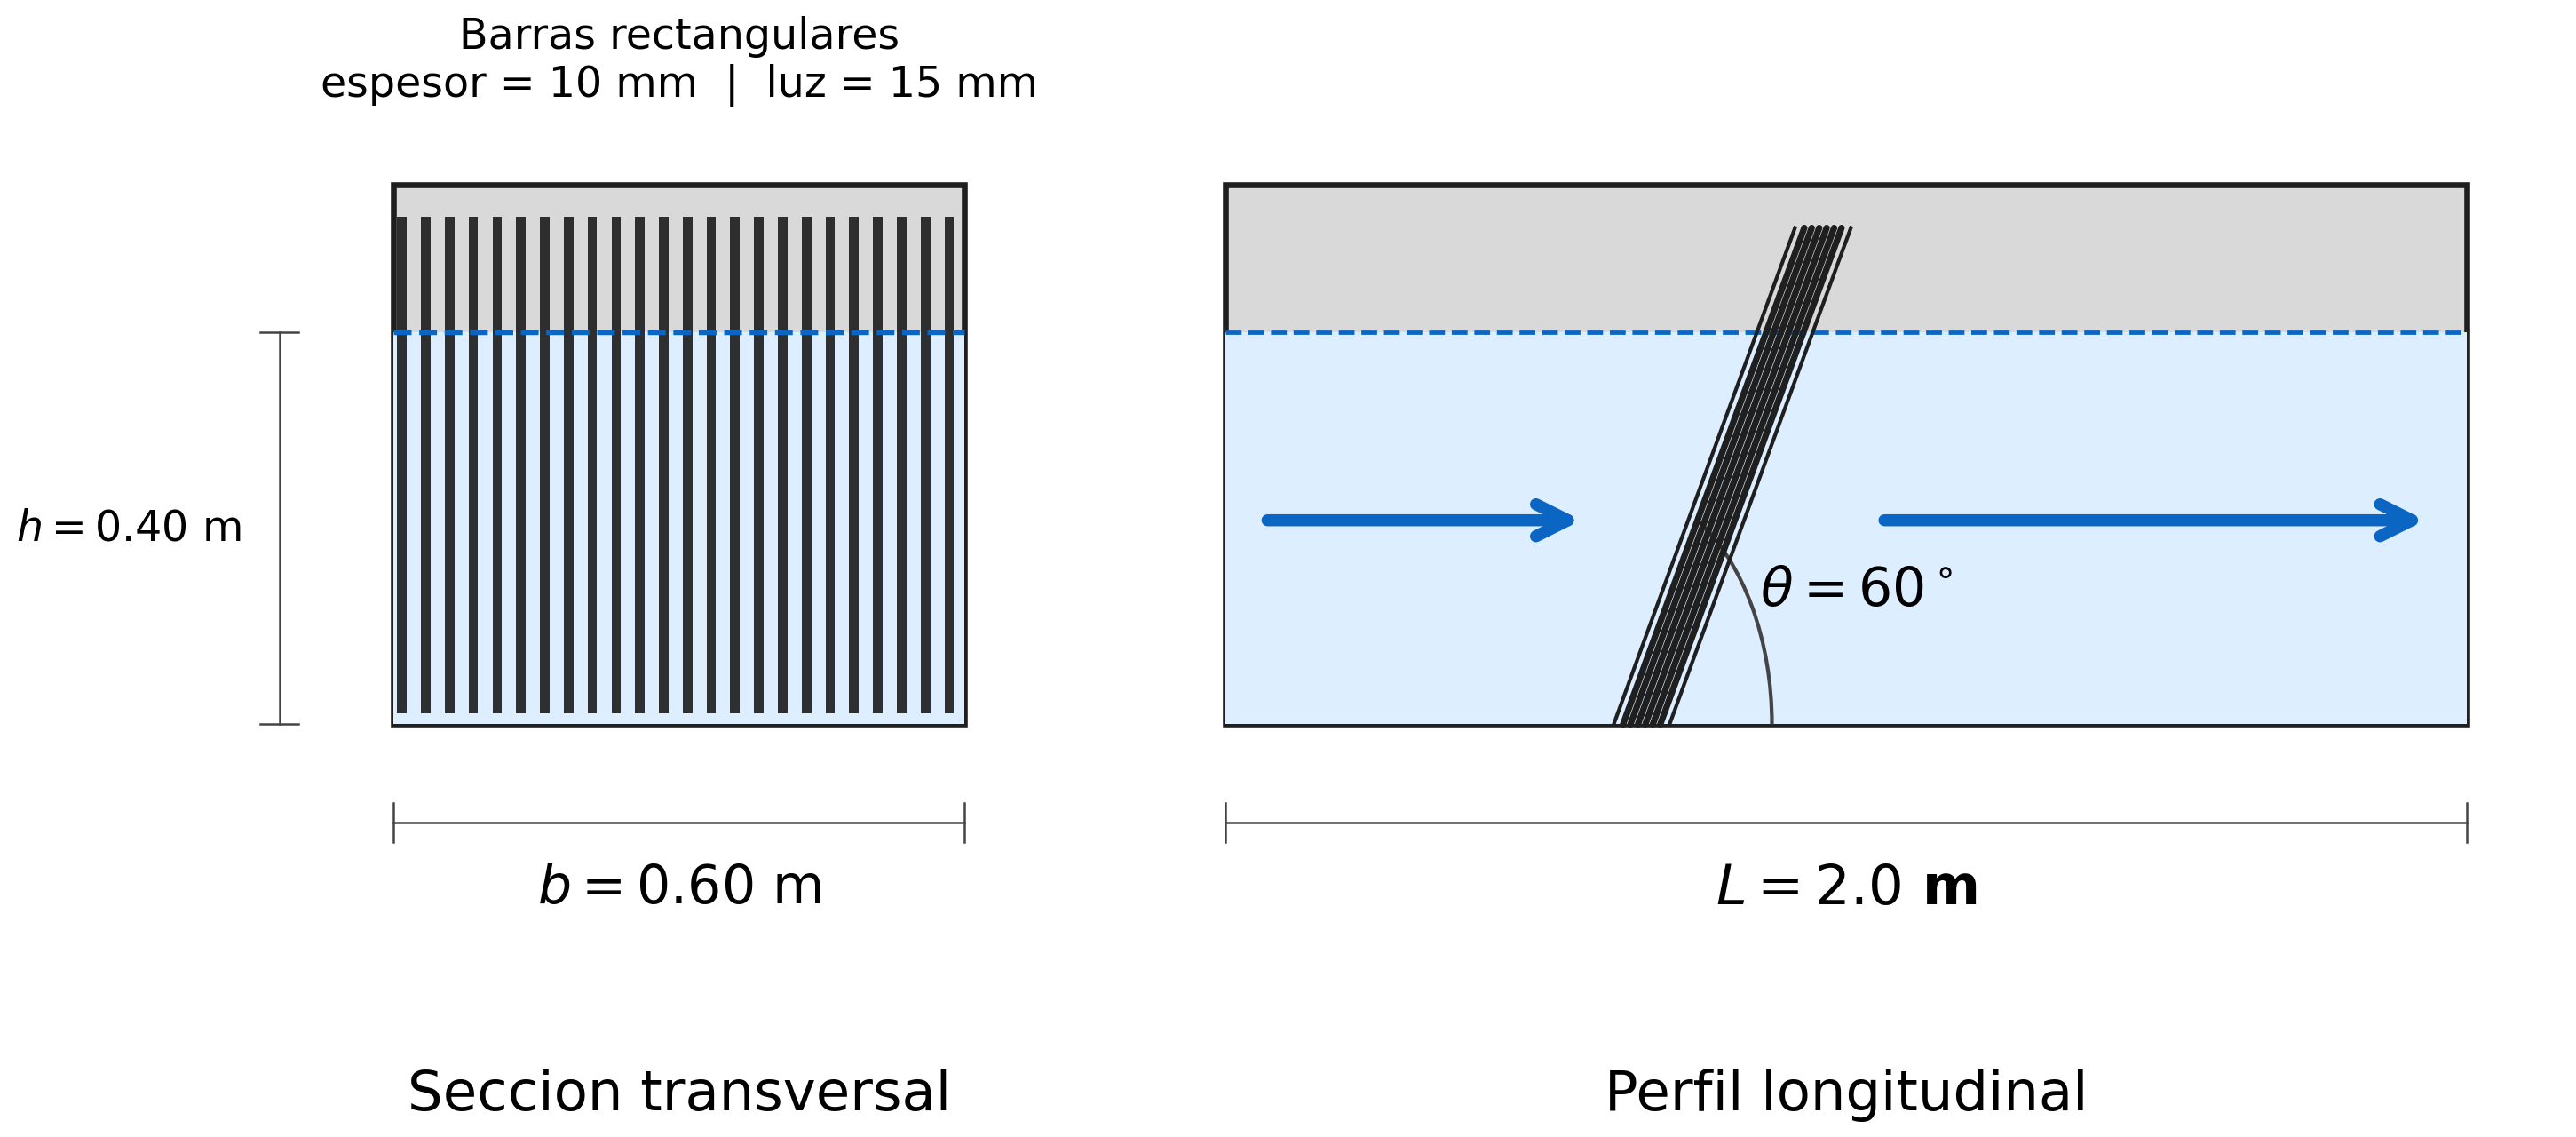
\includegraphics[width=0.9\textwidth]{figuras/rejillas_rejillas.png}
\caption{Esquema del canal de desbaste con rejillas (dimensiones en metros)}
\label{fig:rejillas}
\end{figure}





\textit{Nota sobre cantidades:} El presente dimensionamiento no estima la masa o volumen diario de residuos de cribado. Segun Metcalf y Eddy \cite{metcalf2014}, la produccion tipica de residuos de rejillas finas en aguas residuales municipales varia entre 0.005--0.02 m\textsuperscript{3}/1000 m\textsuperscript{3} de agua tratada. Para el caudal de diseno, esto representaria aproximadamente 0.02--0.09 m\textsuperscript{3}/d (total planta), sujeto a caracterizacion local.

Las dimensiones finales del canal con rejillas son: ancho 0.60 m, tirante 0.40 m y longitud 2.0 m. Se requieren dos unidades, una por cada linea de tratamiento.

\subsection{Desarenador de Flujo Horizontal}



El desarenador remueve part\'iculas minerales (arena, grava) con di\'ametro superior a 0.20~mm mediante sedimentaci\'on gravitacional. Seg\'un Metcalf y Eddy \cite{metcalf2014}, los par\'ametros de dise\~no son: velocidad horizontal 0.25--0.30~m/s (m\'aximo 0.30~m/s para evitar arrastre de sedimentos), tiempo de retenci\'on 30--60~s, y profundidad de flujo 0.75--2.0~m (OPS/CEPIS \cite{ops2005} permite valores menores en plantas peque\~nas).

La profundidad total del canal incluye: profundidad \'util de flujo (0.40~m), zona de almacenamiento de arena (0.25--0.30~m; se adopta 0.30~m), y bordo libre (0.30~m).

El dise\~no del desarenador se fundamenta en la teor\'ia de sedimentaci\'on discreta. Primero se calcula la velocidad de sedimentaci\'on de las part\'iculas objetivo mediante la Ley de Stokes:

\begin{equation}
v_s = \frac{g \cdot (S_s - 1) \cdot d^2}{18 \cdot \nu}
\end{equation}
\captionequation{Ley de Stokes - Velocidad de sedimentacion de particulas}

\textit{Donde:}
\begin{itemize}[noitemsep,leftmargin=2em]
    \item[$v_s$] = Velocidad de sedimentaci\'on (m/s)
    \item[$g$] = Aceleraci\'on de la gravedad (9.81 m/s²)
    \item[$S_s$] = Gravedad espec\'ifica de la arena (2.65)
    \item[$d$] = Di\'ametro de la part\'icula (0.00020 m)
    \item[$\nu$] = Viscosidad cinem\'atica del agua a 25.6°C ($8.3973e-07$ m²/s)
\end{itemize}

\begin{equation}
v_s = \frac{9.81 \times (2.65 - 1) \times (0.00020)^2}{18 \times 8.3973e-07} = 0.043 \text{ m/s}
\end{equation}

Con este valor de $v_s$ se determina la longitud te\'orica del desarenador mediante la ecuaci\'on de sedimentaci\'on tipo I:

\begin{equation}
L = \frac{H \cdot v_h}{v_s} = \frac{0.40 \times 0.30}{0.043} = 2.8 \text{ m}
\end{equation}

\textit{Donde:}
\begin{itemize}[noitemsep,leftmargin=2em]
    \item[$L$] = Longitud del desarenador (m)
    \item[$H$] = Profundidad \'util (0.40 m)
    \item[$v_h$] = Velocidad horizontal adoptada (0.30 m/s)
\end{itemize}

La longitud te\'orica resultante (2.8~m) es adecuada para el caudal de dise\~no y se adopta como longitud de dise\~no.

El ancho del canal se determina por la ecuaci\'on de continuidad:

\begin{equation}
B = \frac{Q}{v_h \cdot H} = \frac{0.00577}{0.30 \times 0.40} = 0.048 \text{ m}
\end{equation}

\textit{Donde:}
\begin{itemize}[noitemsep,leftmargin=2em]
    \item[$B$] = Ancho te\'orico del canal (m)
    \item[$Q$] = Caudal de dise\~no (0.00577 m³/s)
\end{itemize}

El ancho te\'orico resulta inferior al m\'inimo constructivo. Se adopta 0.60 m seg\'un OPS/CEPIS \cite{ops2005} y SENAGUA \cite{senagua2012}, que establecen 0.60 m como ancho m\'inimo para operaci\'on y mantenimiento.

Verificando la velocidad horizontal real con el ancho adoptado:

\begin{equation}
v_{real} = \frac{Q}{B \cdot H} = \frac{0.00577}{0.60 \times 0.40} = 0.024 \text{ m/s}
\end{equation}

El tiempo de retenci\'on real resulta:

\begin{equation}
t_r = \frac{L}{v_{real}} = \frac{3.0}{0.024} = 124.8 \text{ s}
\end{equation}

\subsubsection{Verificacion}

\textbf{Verificacion de Velocidad Critica de Resuspension}

Para garantizar que la arena sedimentada no sea resuspendida por el flujo, se verifica que la velocidad horizontal del dise\~no sea menor que la velocidad cr\'itica de resuspensi\'on, calculada mediante la f\'ormula de Camp-Shields:

\begin{equation}
v_c = \sqrt{\frac{8 \beta g (S_s - 1) d}{f}}
\end{equation}
\captionequation{Velocidad critica de resuspension - Camp-Shields}

\textit{Donde:}
\begin{itemize}[noitemsep,leftmargin=2em]
    \item[$v_c$] = Velocidad cr\'itica de resuspensi\'on (m/s)
    \item[$\beta$] = Factor de forma (0.05, rango 0.04--0.06)
    \item[$g$] = Aceleraci\'on de la gravedad (9.81 m/s²)
    \item[$S_s$] = Gravedad espec\'ifica de la arena (2.65)
    \item[$d$] = Di\'ametro de la part\'icula (0.00020 m)
    \item[$f$] = Factor de fricci\'on de Darcy-Weisbach (0.025, rango 0.02--0.03)
\end{itemize}

\begin{equation}
v_c = \sqrt{\frac{8 \times 0.05 \times 9.81 \times (2.65 - 1) \times 0.00020}{0.025}} = 0.228 \text{ m/s}
\end{equation}
\captionequation{Velocidad critica calculada}

\textbf{Verificacion para Caudal Maximo Horario}

Se verifica el comportamiento hidr\'aulico para el caudal m\'aximo horario, aplicando un factor de pico t\'ipico de 2.8 sobre el caudal medio:

\begin{equation}
Q_{max} = 2.8 \times Q_{medio} = 2.8 \times 5.8 = 16.0 \text{ L/s}
\end{equation}

A caudal m\'aximo, la velocidad horizontal resulta:

\begin{equation}
v_{h,max} = \frac{Q_{max}}{B \cdot H} = \frac{15.983/1000}{0.60 \times 0.40} = 0.067 \text{ m/s}
\end{equation}

El tiempo de retenci\'on a caudal m\'aximo:

\begin{equation}
t_{r,max} = \frac{L}{v_{h,max}} = \frac{3.0}{0.067} = 45.0 \text{ s}
\end{equation}

\textbf{Criterios de verificaci\'on de resuspensi\'on} (Camp-Shields, Metcalf y Eddy \cite{metcalf2014}):

La velocidad calculada $v_{h,max} = 0.067$~m/s se eval\'ua seg\'un (l\'imite: $v_c \times 90\% = 0.205$~m/s):

\begin{equation}
\text{Estado} = \begin{cases}
    \text{SEGURIDAD} & \text{si } v_{h,max} \leq 0.205 \text{ m/s} \quad \text{(no hay resuspensi\'on)} \\
    \text{RIESGO} & \text{si } v_{h,max} > 0.205 \text{ m/s} \quad \text{(arena resuspendida)}
\end{cases}
\end{equation}
\captionequation{Criterios de verificacion de resuspension}

Con la velocidad calculada $v_{h,max} = 0.067$~m/s, la unidad se clasifica como \textbf{SEGURIDAD}. En terminos de cumplimiento, la verificacion de resuspension \textbf{CUMPLE} porque es menor que el limite de resuspension con factor de seguridad (0.205~m/s), por lo que no se produce resuspension de la arena depositada.

\subsubsection{Resultados}

\begingroup
\small
\begin{longtable}{l p{9cm}}
\caption{Dimensiones del desarenador}\\
\toprule
Par\'ametro & Valor \\
\midrule
\endfirsthead
\caption[]{Dimensiones del desarenador (continuación)}\\
\toprule
Par\'ametro & Valor \\
\midrule
\endhead
\midrule
\multicolumn{2}{r}{\textit{Continúa en la siguiente página}} \\
\endfoot
\bottomrule
\endlastfoot
Longitud dise\~no & 3.0 m (m\'inimo constructivo SENAGUA) \\
Ancho & 0.60 m (m\'inimo constructivo) \\
Profundidad \'util & 0.40 m \\
Velocidad horizontal real & 0.024 m/s \\
Velocidad cr\'itica resuspensi\'on & 0.228 m/s (Camp-Shields) \\
Tiempo retenci\'on real & 124.8 s \\
\multicolumn{2}{p{\textwidth}}{\small\textit{$^a$Nota: El TRH de 125~s y velocidad de 0.024~m/s se deben al ancho m\'inimo constructivo de 0.60~m. }} \\
\end{longtable}
\endgroup

\textbf{Manejo de arena removida}

El desarenador retiene part\'iculas minerales, principalmente arena y grava fina, que se sedimentan en el fondo del canal por acci\'on gravitacional. Estas part\'iculas presentan di\'ametros superiores a 0.20~mm, con gravedad espec\'ifica de 2.65, correspondiendo a s\'olidos inorg\'anicos de alta densidad presentes en el agua residual. El canal incorpora una zona de almacenamiento de 0.30~m de altura, dimensionada espec\'ificamente para acumular la arena removida entre operaciones de limpieza. La frecuencia de limpieza recomendada es diaria o seg\'un la acumulaci\'on observada, manteniendo la arena acumulada por debajo del 50\% de la altura de almacenamiento designada para garantizar el funcionamiento \'optimo del sistema. La remoci\'on se realiza manualmente mediante palas y cubos desde la plataforma de operaci\'on, aunque puede implementarse un sistema de succi\'on o bombeo si el caudal y la producci\'on de arena lo justifican t\'ecnicamente.

\textbf{Disposici\'on final de la arena:}

La arena removida en el desarenador puede manejarse de diferentes formas seg\'un su composici\'on y la normativa local vigente. La opci\'on m\'as com\'un es el relleno sanitario, ya que la arena es material inorg\'anico inerte que puede disposicionarse en rellenos autorizados sin restricciones especiales. En caso de que la arena est\'e relativamente limpia, con bajo contenido de materia org\'anica adherida, existe la posibilidad de reuso condicionado para relleno y compactaci\'on en obras civiles previa caracterizaci\'on, mezcla con concreto para elementos no estructurales, o como complemento en sistemas de filtraci\'on gruesa previo lavado. Si se detecta alta carga org\'anica adherida a los granos de arena, evidenciada por olor f\'etido o color oscuro, se recomienda un lavado previo antes de la disposici\'on final para reducir el impacto ambiental.

\begin{figure}[H]
\centering

\includegraphics[width=\textwidth]{figuras/Esquema_Desarenador.png}
\caption{Esquema del desarenador de flujo horizontal con perfil longitudinal y corte transversal. Se muestran la entrada del afluente, la zona de flujo, el dep\'osito de arena y la salida . }
\label{fig:desarenador}
\end{figure}

\textit{Nota sobre cantidades:} El presente dimensionamiento no estima la masa o volumen diario de arena removida. Seg\'un Metcalf y Eddy \cite{metcalf2014}, la producci\'on t\'ipica de arena en aguas residuales municipales var\'ia entre 0.004--0.15 L/m\textsuperscript{3} de agua tratada, dependiendo de las caracter\'isticas del sistema de alcantarillado (red combinada vs. separada) y del suelo local. Para el caudal de dise\'no, esto representar\'ia aproximadamente 0.02--0.6 L/d (total planta), sujeto a caracterizaci\'on local.

\subsection{Reactor Anaerobio con Pantallas (ABR/RAP)}

\subsubsection{Dimensionamiento}

\textbf{Nomenclatura del reactor:} En la literatura técnica internacional, el reactor objeto de este manual se denomina ABR (\textit{Anaerobic Baffled Reactor}). En la literatura hispanohablante y en particular en los manuales de la OPS/OMS para saneamiento en países de desarrollo, se utiliza con frecuencia la sigla RAP (Reactor Anaerobio con Pantallas), que traduce literalmente el mismo concepto. Este documento adopta la denominación ABR como nombre principal del documento y del módulo de cálculo, por ser el término de uso universal en la bibliografía técnica de referencia. La sigla RAP se utiliza en paralelo en los títulos y encabezados del documento —de ahí la denominación compuesta "ABR / RAP"— con el fin de garantizar la trazabilidad con los manuales de la OPS/OMS que sirven de referencia complementaria en este proyecto.

\textbf{¿Qué es un Reactor Anaerobio con Pantallas (ABR / RAP)?}

El Reactor Anaerobio con Pantallas —ABR por sus siglas en inglés— es un sistema de tratamiento biológico anaerobio de aguas residuales que opera mediante flujo a través de una serie de compartimentos separados por pantallas o tabiques verticales (bafles). El agua residual entra por un extremo del reactor y recorre, en serie, cada uno de los compartimentos hasta llegar al extremo opuesto donde descarga el efluente tratado. En cada compartimento, el flujo sigue un patrón alternado de ascenso y descenso determinado por la posición y configuración de las pantallas.

El ABR fue desarrollado y descrito formalmente por McCarty y colaboradores en la Universidad de Stanford (Bachmann et al., 1985) como una evolución simplificada de los reactores anaerobios de lecho de lodos. Su gran ventaja conceptual sobre el reactor UASB (\textit{Upflow Anaerobic Sludge Blanket}) es la ausencia de un separador trifásico: la retención de la biomasa se logra por medios puramente hidráulicos y gravitacionales, aprovechando el hecho de que el flujo ascendente en cada compartimento es suficientemente lento como para mantener el manto de lodos en posición estable.

El ABR ocupa una posición intermedia entre el tanque séptico y el UASB en cuanto a complejidad constructiva y eficiencia de tratamiento. Es más eficiente que el tanque séptico porque el tratamiento ocurre en múltiples etapas en serie, cada una con su propia comunidad microbiana especializada. Es más simple que el UASB porque no requiere el separador trifásico, que es el componente más costoso y delicado de ese reactor. Esta combinación de buena eficiencia y simplicidad constructiva lo convierte en una opción especialmente adecuada para sistemas de saneamiento descentralizados, comunidades rurales y pequeñas cabeceras parroquiales en países de ingresos medios y bajos.

\textbf{Rol en el tren de tratamiento del proyecto:}

En el presente proyecto, el ABR se diseña como unidad de tratamiento primario anaerobio, situada aguas abajo del pretratamiento (cribado y desarenado) y aguas arriba de las unidades de tratamiento complementario o secundario. Su función principal es la remoción de materia orgánica en condiciones anaerobias, la estabilización parcial de los sólidos sedimentables y la acumulación y digestión \textit{in situ} de los lodos generados.

En la configuración típica del proyecto, el ABR reemplaza o complementa al tanque séptico convencional en situaciones donde se requiere un mayor nivel de remoción de DBO y DQO en la etapa anaerobia, con mayor control del proceso y sin la necesidad de un sistema mecánico de aireación. El efluente del ABR puede destinarse a un campo de infiltración, a un humedal de flujo subsuperficial, a un filtro anaerobio de flujo ascendente (FAFA) o, según el nivel de tratamiento requerido, a una etapa de tratamiento aerobio posterior (biofiltro, lodos activados, etc.).

\textbf{Principio de funcionamiento por compartimentos:}

El ABR es un reactor rectangular dividido internamente en una serie de compartimentos por medio de tabiques o pantallas verticales. Los tabiques no llegan completamente al fondo ni completamente a la superficie: dejan aberturas alternadas para forzar el recorrido del agua a través de toda la altura de cada compartimento.

En la configuración adoptada en este proyecto, los tabiques tienen una abertura en la parte inferior. El agua entra por el primer compartimento por el fondo, sube a través de él, desborda por encima del tabique intermedio o pasa por una abertura superior, desciende hasta el fondo del segundo compartimento, vuelve a subir, y así sucesivamente hasta el último compartimento. Este patrón de flujo ascendente-descendente garantiza que el agua atraviese toda la profundidad del manto de lodos en cada compartimento, maximizando el contacto entre el sustrato y la biomasa.

\textbf{Retención de biomasa sin separador trifásico:}

La clave del funcionamiento del ABR es la velocidad ascensional relativamente baja en el interior de cada compartimento. El manto de lodos anaerobio se mantiene en posición porque la velocidad ascendente del flujo no es suficiente para arrastrar los gránulos o flóculos de lodo hacia el compartimento siguiente. Esta retención es fundamentalmente diferente a la del UASB, donde se requiere un separador trifásico para capturar los sólidos que el flujo ascendente tiende a arrastrar hacia la superficie: en el ABR, la propia geometría del sistema asegura que la velocidad ascensional se mantenga por debajo del umbral de arrastre del lodo, sin necesidad de separadores mecánicos adicionales.

La consecuencia práctica es que en el ABR cada compartimento acumula su propia población microbiana, y esa población se adapta progresivamente a la calidad del agua que recibe: el primer compartimento, que recibe el agua cruda más concentrada, contiene predominantemente bacterias hidrolíticas y acidogénicas; los compartimentos intermedios tienen una mezcla de acidogénicos y acetogénicos; y el último compartimento, que recibe un agua ya considerablemente tratada, tiene condiciones más propicias para los metanogénicos. Esta separación funcional a lo largo del reactor es uno de los factores que explican la robustez del ABR frente a variaciones de carga.

\textbf{Mecanismos principales de remoción:}

Los mecanismos de remoción en el ABR son los propios del tratamiento anaerobio en cuatro etapas clásicas:

\textit{Hidrólisis:} Las moléculas orgánicas complejas (proteínas, grasas, hidratos de carbono) son fraccionadas en monómeros y dímeros por enzimas extracelulares producidas por las bacterias hidrolíticas. Esta etapa es generalmente la limitante del proceso para residuales con alta concentración de sólidos particulados.

\textit{Acidogénesis:} Los productos de la hidrólisis son fermentados por bacterias acidogénicas a ácidos grasos volátiles (AGV), alcoholes, dióxido de carbono e hidrógeno. Esta etapa es generalmente rápida en comparación con la hidrólisis y con la metanogénesis.

\textit{Acetogénesis:} Los ácidos grasos volátiles de cadena corta (propionato, butirato) son convertidos a acetato, CO$_2$ e H$_2$ por bacterias acetogénicas. Esta etapa es termodinámicamente desfavorable a concentraciones altas de H$_2$ y solo ocurre de forma eficiente cuando el hidrógeno es consumido rápidamente por organismos hidrogenotróficos (sintrofía obligada).

\textit{Metanogénesis:} El acetato y el H$_2$/CO$_2$ son convertidos a metano y CO$_2$ por las arqueas metanogénicas. Esta etapa es la más sensible a variaciones de pH y temperatura, y la que limita la tasa global del proceso cuando el sistema está correctamente operado.

Adicionalmente, en el ABR ocurre sedimentación de sólidos suspendidos por efecto de la reducción de velocidad dentro de cada compartimento: los sólidos gruesos que no se degradan rápidamente sedimentan en el fondo del primer compartimento o de los primeros compartimentos, donde se acumulan y se digieren lentamente. Esta función es análoga a la del tanque séptico, pero con la ventaja de que el tratamiento biológico activo ocurre en paralelo y de forma mucho más eficiente.

\textbf{Criterios de diseño adoptados por el proyecto:}

Los siguientes parámetros han sido seleccionados como criterios de diseño para el reactor ABR, basados en la bibliografía técnica y adaptados a las condiciones del proyecto:

\begin{table}[H]
\centering
\caption{Parámetros seleccionados para el diseño ABR / RAP}
\begin{tabular}{p{6cm}cc}
\toprule
\textbf{Parámetro} & \textbf{Valor adoptado} & \textbf{Rango recomendado} \\
\midrule
Tiempo de retención hidráulico (TRH) & 24 h & 24--72 h \\
Número de compartimentos ($n$) & 4 & 2--8 (recomendado: 4--6) \\
Velocidad ascensional de diseño ($v_{up}$) & 1.0 m/h & 0,2--1,5 m/h \\
Profundidad útil del líquido ($H$) & 2.0 m & 1,5--3,0 m \\
Zona de acumulación de lodos & 0.30 m & 0,2--0,5 m \\
Bordo libre & 0.30 m & $\geq$ 0,30 m \\
\bottomrule
\end{tabular}
\end{table}

\textit{Nota: Estos valores son criterios adoptados por el proyecto basados en Barber \& Stuckey (1999), Foxon et al. (2004) y OPS/OMS (2005). No son límites normativos impuestos por la TULSMA ni por normas ecuatorianas específicas para reactores anaerobios.}

\textbf{Ecuaciones de dimensionamiento:}

El dimensionamiento del ABR se fundamenta en el criterio del tiempo de retención hidráulico (TRH) y en la verificación de la velocidad ascensional. Las ecuaciones fundamentales son las siguientes:

\textbf{[Ecuación 1] Volumen total del reactor:}

\begin{equation}
V_{total} = Q_{medio} \times TRH
\end{equation}

\textit{Donde:}
\begin{itemize}[noitemsep,leftmargin=2em]
    \item[$V_{total}$] = Volumen total del reactor (m³)
    \item[$Q_{medio}$] = Caudal medio diario de diseño (498.5 m³/d = 20.77 m³/h)
    \item[$TRH$] = Tiempo de retención hidráulico adoptado (24 h = 1.00 d)
\end{itemize}

Sustituyendo los valores del proyecto:

\begin{equation}
V_{total} = 498.5 \times 1.000 = 498.5 \text{ m}^3
\end{equation}

\textbf{[Ecuación 2] Volumen por compartimento:}

\begin{equation}
V_{comp} = \frac{V_{total}}{n} = \frac{498.5}{4} = 124.63 \text{ m}^3
\end{equation}

\textbf{[Ecuación 3] Área de sección transversal por velocidad ascensional:}

La velocidad ascensional es el parámetro crítico que controla la retención de la biomasa en el reactor. Para que el ABR funcione correctamente, la velocidad ascensional debe ser inferior a la velocidad de sedimentación de los flóculos de lodo.

\begin{equation}
A_{transversal} = \frac{Q_{medio}}{v_{up, dise\tilde{n}o}} = \frac{20.77}{1.0} = 20.77 \text{ m}^2
\end{equation}

\textbf{[Ecuación 4] Dimensiones del reactor:}

A partir del área de sección transversal y la profundidad útil adoptada, se obtienen las dimensiones geométricas:

\begin{equation}
W = \frac{A_{transversal}}{H} = \frac{20.77}{2.0} = 10.39 \text{ m} \quad \text{(ancho)}
\end{equation}

\begin{equation}
L_{comp} = \frac{V_{comp}}{W \times H} = \frac{124.63}{10.39 \times 2.0} = 6.00 \text{ m} \quad \text{(largo por compartimento)}
\end{equation}

\begin{equation}
L_{total} = n \times L_{comp} = 4 \times 6.00 = 24.00 \text{ m} \quad \text{(largo total)}
\end{equation}

La profundidad total de construcción incluye la profundidad útil del líquido, la zona de acumulación de lodos y el bordo libre:

\begin{equation}
H_{total} = H + H_{lodos} + H_{bordo} = 2.0 + 0.30 + 0.30 = 2.60 \text{ m}
\end{equation}

\textbf{[Ecuación 5] Altura de abertura en los bafles (slot inferior):}

Cada pantalla o bafle interno no ocupa toda la altura del compartimento: deja una abertura en su parte inferior (slot) por la que el flujo debe pasar antes de ascender en el compartimento siguiente. La altura de este slot es un parámetro de diseño que determina la velocidad puntual del flujo en la transición entre compartimentos. Según OPS/OMS (2005) y Foxon et al. (2004), esta abertura se define como una fracción de la profundidad útil, típicamente entre el 15\,\% y el 25\,\% de $H$. Adoptando el valor central de la bibliografía ($f_{slot} = 0.20$):

\begin{equation}
h_{slot} = f_{slot} \times H = 0.20 \times 2.0 = 0.40 \text{ m}
\end{equation}

\textbf{[Ecuación 6] Velocidad en la abertura de los bafles:}

La velocidad del flujo al atravesar la abertura inferior de cada bafle (\textit{slot velocity}) es significativamente mayor que la velocidad ascensional media del compartimento, porque el área de paso queda reducida a $W \times h_{slot}$. Este parámetro es crítico: un valor excesivo genera turbulencia local en el fondo del compartimento siguiente, resuspende los lodos sedimentados y puede provocar su arrastre hacia el efluente. La bibliografía recomienda mantener esta velocidad por debajo de 1.0~m/h a caudal medio:

\begin{equation}
v_{slot} = \frac{Q_{medio}}{W \times h_{slot}} = \frac{20.770}{10.39 \times 0.40} = 5.00 \text{ m/h}
\end{equation}

\textbf{Limitaciones del método actual:}

El presente dimensionamiento cubre el cálculo del volumen total, número y tamaño de compartimentos, geometría del reactor, verificaciones hidráulicas y parámetros de carga. No cubre, en esta versión del cálculo: el modelado de la eficiencia de remoción de DBO en función del TRH (que requeriría un modelo cinético calibrado), el cálculo de la producción de biogás, el diseño del sistema de ventilación del biogás, el balance detallado de lodos en estado estacionario, ni el dimensionamiento de tuberías de entrada, salida y extracción de lodos.

\subsubsection{Verificación}

La subsección de verificación evalúa de forma sistemática si el reactor dimensionado satisface los criterios hidráulicos y geométricos de la bibliografía de referencia. Para cada verificación se describe primero el fenómeno físico que la motiva, después se desarrolla el cálculo con los valores del proyecto y, finalmente, se emite el juicio de cumplimiento. Se distinguen verificaciones \textbf{obligatorias} ---cuyo incumplimiento invalida el diseño--- de \textbf{complementarias} ---que orientan sobre la calidad del diseño sin invalidarlo--- y de \textbf{parámetros informativos} ---que no tienen criterio de cumplimiento en este nivel de diseño---.

\textbf{Verificaciones obligatorias:}

\textbf{[V-1] Rango bibliográfico de la velocidad ascensional de diseño}

El primer parámetro que debe justificarse es la propia elección de la velocidad ascensional de diseño $v_{up,dise\tilde{n}o} = 1.0$~m/h. Este valor no es un resultado del cálculo sino una decisión del proyectista: determina el área transversal del reactor (Ecuación~3) y, a través de ella, todas las demás dimensiones geométricas. Su validez depende de que se encuentre dentro del rango operativo aceptable reportado en la bibliografía técnica.

Las razones de este límite son físicas: velocidades demasiado altas generan shear suficiente para arrastrar los flóculos de lodo anaerobio hacia el efluente, empobreciendo progresivamente la biomasa activa del reactor; velocidades demasiado bajas producen reactores sobredimensionados sin mejora proporcional en la eficiencia biológica, pues el limitante del proceso pasa a ser la cinética de la metanogénesis y no el tiempo de contacto. Según Foxon et al. (2004) y Barber \& Stuckey (1999), el rango operativo aceptable para aguas residuales domésticas a temperatura ambiente es:

\begin{equation}
0.2 \text{ m/h} \leq v_{up,dise\tilde{n}o} \leq 1.5 \text{ m/h}
\end{equation}

El valor adoptado en este proyecto es $v_{up,dise\tilde{n}o} = 1.0$~m/h.

\textit{Nota importante sobre la verificación de la velocidad a caudal medio:} la velocidad ascensional calculada a caudal medio ($v_{up,calc} = Q_{medio} / (W \times H)$) coincide por construcción con $v_{up,dise\tilde{n}o}$, puesto que el ancho $W$ se obtuvo directamente como $W = Q_{medio} / (v_{up,dise\tilde{n}o} \times H)$. No existe por tanto una verificación numérica independiente a caudal medio: la verificación real y crítica de la velocidad ascensional es la del caudal pico (V-2), que sí puede superar el límite admisible.

Estado V-1: \textbf{CUMPLE} ($0.2 \leq 1.0 \leq 1.5$~m/h)

\textbf{[V-2] Velocidad ascensional a caudal máximo horario}

Esta es la verificación hidráulica más crítica del diseño. Durante los picos de consumo ---generalmente en las mañanas y mediodías en sistemas domésticos--- el caudal supera al medio en un factor de pico $f_p$. Si en esas condiciones la velocidad ascensional rebasa el umbral de arrastre, la biomasa abandona el reactor con el efluente y el rendimiento de depuración se deteriora progresivamente. A diferencia del UASB, el ABR carece de separador trifásico que retenga los sólidos en esas condiciones: la única salvaguarda es que la geometría garantice una velocidad admisible incluso en pico.

El caudal pico horario se obtiene aplicando el factor de pico al caudal medio de diseño:

\begin{equation}
Q_{max} = f_p \times Q_{medio} = 2.8 \times 20.770 = 57.540 \text{ m}^3\text{/h}
\end{equation}

Con este caudal, la velocidad ascensional en pico resulta:

\begin{equation}
v_{up,max} = \frac{Q_{max}}{W \times H} = \frac{57.540}{10.39 \times 2.0} = 2.77 \text{ m/h}
\end{equation}

El límite bibliográfico para caudal pico, según Barber \& Stuckey (1999), es de 2.0~m/h. Por encima de este umbral se ha observado exportación significativa de sólidos hacia el efluente en reactores piloto y a escala real.

Criterio: $v_{up,max} \leq 2.0$~m/h

Estado V-2: \textbf{NO CUMPLE} (2.77~m/h $>$ 2.0~m/h)

\textbf{[V-3] Verificación del tiempo de retención hidráulico por geometría}

El TRH de diseño fija el volumen total del reactor (Ecuación~1). Sin embargo, las dimensiones finales resultan de una cadena de operaciones aritméticas ---división por área, multiplicación por número de compartimentos--- que en la práctica pueden ajustarse a valores constructivos enteros. Esta verificación confirma que el volumen efectivo de la geometría adoptada reproduce, o supera, el TRH de diseño. Si el TRH calculado resultara inferior al de diseño, significaría que las dimensiones son insuficientes y que el tiempo de contacto nominal no se alcanzaría en la práctica.

\begin{equation}
TRH_{calc} = \frac{L_{total} \times W \times H_{util}}{Q_{medio}} \times 24 = \frac{24.00 \times 10.39 \times 2.0}{498.5} \times 24 = 24.0 \text{ h}
\end{equation}

Criterio: $TRH_{calc} \geq 24$~h

Estado V-3: \textbf{CUMPLE} (24.0~h $\geq$ 24~h)

\textbf{[V-4] Largo mínimo de compartimento}

El largo de cada compartimento ($L_{comp}$) debe satisfacer dos criterios independientes que responden a razones diferentes. El criterio constructivo establece un mínimo absoluto de 1.0~m: por debajo de esta dimensión el compartimento es impracticable desde el punto de vista de la ejecución de obra, la inspección y la extracción de lodos. El criterio hidráulico-bibliográfico, según OPS/OMS (2005), establece que $L_{comp} \geq H_{util}$: esta condición garantiza que el recorrido horizontal del flujo sea suficiente para que los sólidos gruesos no degradados sedimenten antes de alcanzar el bafle siguiente, evitando cortocircuitos hidráulicos. Ambos criterios deben cumplirse simultáneamente, por lo que el largo mínimo efectivo es el mayor de los dos valores:

\begin{equation}
L_{comp,min} = \max\!\left(H_{util},\; 1.0\right) = \max\!\left(2.0,\; 1.0\right) = 2.0 \text{ m}
\end{equation}

Valor calculado: $L_{comp} = 6.00$~m

Estado V-4: \textbf{CUMPLE} ($L_{comp} = 6.00$~m $\geq$ 2.0~m)

\textbf{[V-5] Velocidad en la abertura inferior de los bafles (\textit{slot velocity})}

Cada pantalla interna del ABR deja una abertura en su parte inferior (denominada \textit{slot} en la bibliografía anglosajona) a través de la cual el flujo pasa de un compartimento al siguiente antes de ascender. Dado que el área de esta abertura ($W \times h_{slot}$) es sustancialmente menor que el área transversal total del compartimento ($W \times H$), la velocidad puntual del flujo en el slot es notablemente mayor que la velocidad ascensional media.

Esta aceleración local tiene dos efectos negativos cuando supera el umbral admisible: primero, genera turbulencia en el fondo del compartimento receptor, resuspendiendo los flóculos de lodo ya sedimentados; segundo, puede crear zonas de mezcla intensa que cortocircuitan la separación funcional entre compartimentos, que es uno de los fundamentos del buen rendimiento del ABR. OPS/OMS (2005) y Foxon et al. (2004) recomiendan definir la abertura como el 20\,\% de la profundidad útil ($f_{slot} = 0.20$) y mantener la velocidad en el slot por debajo de 1.0~m/h a caudal medio:

\begin{equation}
h_{slot} = f_{slot} \times H_{util} = 0.20 \times 2.0 = 0.40 \text{ m}
\end{equation}

La velocidad en la abertura a caudal medio resulta:

\begin{equation}
v_{slot} = \frac{Q_{medio}}{W \times h_{slot}} = \frac{20.770}{10.39 \times 0.40} = 5.00 \text{ m/h}
\end{equation}

A modo informativo, a caudal máximo:

\begin{equation}
v_{slot,max} = \frac{Q_{max}}{W \times h_{slot}} = \frac{57.540}{10.39 \times 0.40} = 13.85 \text{ m/h}
\end{equation}

Criterio: $v_{slot} \leq 1.0$~m/h (caudal medio)

Estado V-5: \textbf{NO CUMPLE} (5.00~m/h $>$ 1.0~m/h)

\textbf{[V-6] Relación profundidad útil / ancho del reactor ($H/W$)}

La relación $H/W$ describe la forma de la sección transversal de cada compartimento. Su importancia es reconocida en la bibliografía reciente (Sinha et al., 2009): valores extremos en cualquier sentido comprometen la uniformidad del flujo vertical ascendente. Un reactor excesivamente ancho en relación con su profundidad ($H/W < 0.5$) tiende a tener distribución no uniforme del flujo en el plano transversal, con zonas muertas en los extremos laterales donde la velocidad ascensional es insuficiente para mantener el manto de lodos en suspensión activa. Por el contrario, un reactor excesivamente estrecho ($H/W > 2.0$) dificulta la distribución uniforme del afluente en el ancho y puede crear flujos preferenciales en la zona central que reducen el contacto efectivo entre el sustrato y la biomasa. El rango recomendado es:

\begin{equation}
0.5 \leq \frac{H_{util}}{W} \leq 2.0
\end{equation}

El valor calculado para este diseño es:

\begin{equation}
\frac{H_{util}}{W} = \frac{2.0}{10.39} = 0.19
\end{equation}

Estado V-6: \textbf{NO CUMPLE} ($0.5 \leq 0.19 \leq 2.0$)

\textbf{Verificaciones complementarias:}

\textbf{[V-7] Relación largo / ancho del compartimento ($L_{comp} / W$)}

La relación $L_{comp} / W$ describe la esbeltez en planta de cada compartimento. Compartimentos muy alargados ($L_{comp} / W > 2.0$) pueden presentar distribución no uniforme del afluente a lo largo del ancho; compartimentos muy cuadrados o anchos ($L_{comp} / W < 0.5$) tienden hacia un comportamiento de mezcla completa en el plano horizontal, reduciendo la eficiencia de la separación en serie entre compartimentos. El rango orientativo recomendado por la OPS/OMS (2005) es:

\begin{equation}
0.5 \leq \frac{L_{comp}}{W} \leq 2.0
\end{equation}

Valor calculado: $L_{comp} / W = 6.00 / 10.39 = 0.58$

Estado V-7: \textbf{DENTRO RANGO} (verificación complementaria)

\textbf{[V-8] Número mínimo de compartimentos}

El número de compartimentos determina el grado de separación funcional entre las fases del proceso anaerobio. Con un solo compartimento el ABR no tiene ventaja sobre un digestor de mezcla completa. A partir de cuatro compartimentos se logra una separación razonablemente clara entre las comunidades hidrolítico-acidogénicas (primer y segundo compartimento) y las metanogénicas (últimos compartimentos). La OPS/OMS (2005) establece un mínimo de 3 compartimentos para aplicaciones de saneamiento doméstico descentralizado:

\begin{equation}
n \geq 3
\end{equation}

Valor adoptado: $n = 4$

Estado V-8: \textbf{CUMPLE}

\textbf{Parámetros informativos:}

\textbf{[V-9] Carga orgánica volumétrica (COV)}

La carga orgánica volumétrica expresa la cantidad de materia orgánica que ingresa por unidad de volumen y por día. Es el parámetro de referencia más utilizado en la bibliografía de reactores anaerobios para comparar diseños y evaluar si el reactor opera en un régimen compatible con el mantenimiento de una biomasa estable. No constituye un criterio obligatorio en este diseño, pero permite situar el proyecto en el contexto de experiencias reportadas.

La DBO se expresa en mg/L, unidad equivalente a g/m³; dividirla entre 1\,000 convierte g a kg. La expresión completa con sus unidades explícitas es:

\begin{equation}
COV = \frac{Q_{medio} \,[\text{m}^3/\text{d}] \times DBO_{entrada} \,[\text{g/m}^3] \,/\, 1\,000}{V_{total} \,[\text{m}^3]} = \frac{498.5 \times 231 / 1\,000}{498.5} = 0.23 \text{ kg\,DBO/(m}^3\!\cdot\!\text{d)}
\end{equation}

Rango bibliográfico para ABR doméstico a temperatura ambiente: 0.5--5.0~kg\,DBO/(m³·d) (Barber \& Stuckey, 1999; OPS/OMS, 2005).

\textbf{[V-10] Estimación de la producción de lodos y frecuencia de purga}

La zona de acumulación de lodos reservada en el dimensionamiento ($H_{lodos} = 0.30$~m) debe ser coherente con la tasa real de producción de biomasa anaerobia en el reactor. Sin esta comprobación, el espacio reservado para lodos es solo un criterio empírico desconectado de las condiciones reales del proyecto. La OPS/OMS (2005, Capítulo~6) proporciona la siguiente expresión para una estimación de orden de magnitud:

\begin{equation}
P_{lodos} = Y_{obs} \times DBO_{rem}
\end{equation}

Donde $Y_{obs} \approx 0.10$~kg\,SSV/kg\,DBO\,removida es el rendimiento observado en digestión anaerobia mesofílica de aguas residuales domésticas (Rittmann \& McCarty, 2001), y $DBO_{rem}$ es la DBO removida diariamente. Adoptando la eficiencia de referencia bibliográfica del 75\,\%:

\begin{equation}
DBO_{rem} = \eta_{ref} \times DBO_{entrada} \times \frac{Q_{medio}}{1\,000} = 0.75 \times 231 \times \frac{498.5}{1\,000} = 86.35 \text{ kg\,DBO/d}
\end{equation}

\begin{equation}
P_{lodos} = 0.10 \times 86.35 = 8.63 \text{ kg\,SSV/d}
\end{equation}

Adoptando una densidad de lodos húmedos anaerobios espesados de $\rho = 1\,040$~kg/m³, el volumen acumulado anualmente es:

\begin{equation}
V_{lodos,año} = \frac{P_{lodos} \times 365}{\rho} = \frac{8.63 \times 365}{1\,040} = 3.03 \text{ m}^3\text{/año}
\end{equation}

El volumen disponible en la zona de lodos del reactor es:

\begin{equation}
V_{zona\,lodos} = L_{total} \times W \times H_{lodos} = 24.00 \times 10.39 \times 0.30 = 74.81 \text{ m}^3
\end{equation}

Esto implica una frecuencia indicativa de purga de lodos de aproximadamente \textbf{237 meses}, asumiendo extracción cuando la zona de acumulación alcanza el 80\,\% de su capacidad. Este valor es una estimación de orden de magnitud y deberá ajustarse en la puesta en marcha del sistema en función de las mediciones reales de producción de lodos.

\textbf{Resumen de verificaciones:}

\begin{table}[H]
\centering
\caption{Resumen de verificaciones del reactor ABR / RAP}
\begin{tabular}{llp{5.5cm}}
\toprule
\textbf{Verificación} & \textbf{Estado} & \textbf{Valor calculado vs. criterio} \\
\midrule
V-1 Rango v\_up diseño & \checkmark & 1.0 m/h $\in$ [0.2--1.5] m/h \\
V-2 v\_up caudal máximo & \texttimes & 2.77 m/h $\leq$ 2.0 m/h \\
V-3 TRH verificado & \checkmark & 24.0 h $\geq$ 24 h \\
V-4 Largo mínimo compartimento & \checkmark & L\_comp = 6.00 m $\geq$ 2.0 m \\
V-5 Velocidad abertura bafle & \texttimes & 5.00 m/h $\leq$ 1.0 m/h \\
V-6 Relación H/W & \texttimes & 0.19 $\in$ [0.5--2.0] \\
\bottomrule
\end{tabular}
\end{table}

\textbf{ATENCIÓN:} las siguientes verificaciones NO cumplen y requieren revisión del diseño: V-2 v\_up caudal máximo, V-5 Velocidad abertura bafle, V-6 Relación H/W.

\textit{Notas: (a) El proyecto NO calcula la eficiencia de remoción de DBO a partir de parámetros operacionales. Las eficiencias del 70--95\,\% reportadas en la bibliografía para ABR con TRH de 24~h son referencias y no predicciones garantizadas. (b) La estimación de producción de lodos (V-10) adopta una eficiencia de referencia del 75\,\%; el valor real dependerá de las condiciones de operación.}

\subsubsection{Resultados}

\begin{figure}[H]
\centering

\includegraphics[width=0.95\textwidth]{figuras/Esquema_ABR.png}
\caption{Esquema del Reactor Anaerobio con Pantallas (ABR / RAP) -- vista longitudinal}
\label{fig:esquema_abr}
\end{figure}

El dimensionamiento del Reactor Anaerobio con Pantallas (ABR / RAP) ha producido las siguientes dimensiones y parámetros de operación:

El esquema muestra la configuración típica del ABR con flujo en zigzag (\textit{up-flow} y \textit{down-flow}) a través de los compartimentos, las pantallas internas (\textit{baffles}) que dirigen el flujo, las zonas de lodos, líquida y biogás, así como los puntos de entrada, salida y ventilación.

\begin{longtable}{p{6cm}p{3cm}p{5cm}}
\caption{Resultados del dimensionamiento ABR / RAP} \\
\toprule
\textbf{Parámetro} & \textbf{Valor} & \textbf{Observación} \\
\midrule
\endfirsthead
\multicolumn{3}{c}{
    {\bfseries \tablename\ \thetable{} -- continuación de la página anterior}
} \\
\toprule
\textbf{Parámetro} & \textbf{Valor} & \textbf{Observación} \\
\midrule
\endhead
\midrule
\multicolumn{3}{r}{Continúa en la siguiente página...} \\
\endfoot
\bottomrule
\endlastfoot

\multicolumn{3}{l}{\textit{Parámetros de entrada:}} \\
Caudal medio ($Q_{medio}$) & 498.5 m³/d & Caudal por línea de tratamiento \\
Caudal máximo ($Q_{max}$) & 1380.9 m³/d & Factor pico: 2.8 \\
DBO afluente & 231 mg/L & Caracterización afluente \\
\midrule

\multicolumn{3}{l}{\textit{Criterios de diseño adoptados:}} \\
Tiempo retención hidráulico (TRH) & 24 h & Criterio del proyecto \\
Número de compartimentos ($n$) & 4 & 4--8 recomendado \\
Velocidad ascensional diseño & 1.0 m/h & $\leq$ 2.0 m/h límite pico \\
Profundidad útil ($H$) & 2.0 m & 1.5--3.0 m rango \\
\midrule

\multicolumn{3}{l}{\textit{Dimensiones geométricas:}} \\
Volumen total ($V_{total}$) & 498.5 m³ & Calculado por TRH \\
Volumen por compartimento & 124.63 m³ & Distribución uniforme \\
Área sección transversal & 20.77 m² & Por velocidad ascensional \\
Ancho del reactor ($W$) & 10.39 m & Geometría transversal \\
Largo por compartimento & 6.00 m & $L_{comp} \geq H$ verificado \\
Largo total ($L_{total}$) & 24.00 m & $n \times L_{comp}$ \\
Profundidad total construcción & 2.60 m & $H + H_{lodos} + H_{bordo}$ \\
Área en planta total & 249.26 m² & $L_{total} \times W$ \\
\midrule

\multicolumn{3}{l}{\textit{Parámetros hidráulicos:}} \\
Velocidad ascensional (caudal medio) & 1.00 m/h & CUMPLE \\
Velocidad ascensional (caudal máximo) & 2.77 m/h & NO CUMPLE \\
TRH calculado & 24.0 h & CUMPLE \\
Carga hidráulica superficial (CHS) & 2.00 m/d & Parámetro informativo \\
\midrule

\multicolumn{3}{l}{\textit{Parámetros de proceso (informativos):}} \\
Carga orgánica volumétrica (COV) & 0.23 kg/m³·d & Rango ref: 0.5--5.0 \\
\midrule

\multicolumn{3}{l}{\textit{Estado de verificaciones:}} \\
Verificación velocidad (medio) & CUMPLE & Criterio: $\leq$ 1.0 m/h \\
Verificación velocidad (máx) & NO CUMPLE & Criterio: $\leq$ 2.0 m/h \\
Verificación TRH & CUMPLE & Criterio: $\geq$ 24 h \\
Verificación largo comp. & CUMPLE & Criterio: $L_{comp} \geq H$ \\
\bottomrule
\multicolumn{3}{l}{\textbf{Estado general del diseño:} \textbf{REQUIERE REVISIÓN}} \\
\end{longtable}

\textbf{Notas sobre los resultados:}

El reactor ABR / RAP dimensionado consta de 4 compartimentos idénticos con una geometría rectangular de 24.00~m de largo total, 10.39~m de ancho y 2.60~m de profundidad total de construcción. La profundidad útil del líquido es de 2.0~m, con una zona adicional de 0.30~m reservada para acumulación de lodos y 0.30~m de bordo libre.

El diseño opera con una velocidad ascensional de 1.00~m/h a caudal medio, valor que se eleva hasta 2.77~m/h durante los picos de caudal. La velocidad a caudal medio cumple con el límite operativo, pero la velocidad de pico supera el umbral bibliográfico admisible (2.0~m/h), lo que indica que el reactor puede experimentar arrastre de biomasa en condiciones de caudal máximo y debe ser revisado.

El tiempo de retención hidráulico de 24.0~h (1.00~días) proporciona el tiempo de contacto necesario entre el agua residual y la biomasa anaerobia para la degradación de la materia orgánica. Este valor se encuentra dentro del rango recomendado de 24--72 horas para reactores ABR tratando aguas residuales domésticas.

\textbf{Alcance y limitaciones declaradas:}

Este dimensionamiento cubre el volumen del reactor, la geometría básica y las verificaciones hidráulicas fundamentales. No incluye: (a) predicción de la eficiencia de remoción de DBO o DQO mediante modelos cinéticos; (b) cálculo de la producción de biogás ni dimensionamiento del sistema de ventilación; (c) balance detallado de producción de lodos y frecuencia de extracción; (d) diseño de las pantallas internas (altura, espesor, configuración de aberturas); (e) dimensionamiento de tuberías de entrada, salida y extracción de lodos. Estos elementos constituyen extensiones futuras del diseño que deben desarrollarse según las condiciones específicas del proyecto.

\subsection{Humedal Artificial de Flujo Vertical (HAFV)}




El Humedal Artificial de Flujo Vertical (HAFV) es un sistema de tratamiento biológico extensivo en el que el agua residual percola verticalmente a través de un medio filtrante granular estratificado, dentro del cual se desarrolla una biopelícula microbiana densa responsable de la degradación de la materia orgánica carbonácea y la oxidación del nitrógeno amoniacal. A diferencia de los sistemas de flujo horizontal subsuperficial (HFHS), donde el agua atraviesa el lecho en sentido horizontal y predominan condiciones anóxicas, el HAFV opera en modo intermitente, alternando períodos de saturación del medio con períodos de drenaje y re-aireación natural. Este ciclo es el mecanismo fundamental que distingue al sistema y le confiere sus características de rendimiento.

Durante el pulso de alimentación, el agua residual se distribuye uniformemente sobre la superficie del filtro mediante un sistema de tuberías perforadas y percola gravitacionalmente hacia la capa de drenaje inferior. Durante este tránsito, los microorganismos del biofilm oxidan la materia orgánica en condiciones aerobias, consumen el oxígeno disuelto remanente y promueven la nitrificación del amonio. Concluido el pulso, el medio drena libremente y el aire penetra desde los tubos de ventilación del fondo y desde la superficie, restaurando las condiciones aerobias en el interior del lecho. Esta re-aireación pasiva, que ocurre sin ningún aporte de energía, es el rasgo que hace al HAFV un sistema energéticamente eficiente y operativamente robusto.

La vegetación macrófita (\textit{Phragmites australis} o equivalentes tropicales) que se establece sobre el lecho cumple una función auxiliar pero no menor: su sistema radicular crea micrositios aerobios en la zona superficial del medio, transfiere pequeñas cantidades de oxígeno hacia la rizosfera, previene la compactación de las capas superiores y contribuye al soporte estructural del lecho filtrante. Su contribución directa a la remoción de contaminantes es secundaria respecto a la actividad del biofilm, pero su rol en la estabilidad física y biológica del sistema a largo plazo es fundamental.

Los mecanismos de remoción de contaminantes en el HAFV, sus eficiencias típicas y los parámetros responsables se resumen en la Tabla~\ref{tab:mecanismos_hafv}.

\begin{table}[H]
\centering
\caption{Mecanismos de remoción y eficiencias típicas en el HAFV (Kadlec \& Wallace, 2009; Cooper et al., 1996)}
\label{tab:mecanismos_hafv}
\begin{tabular}{p{2.2cm}p{6.5cm}cc}
\toprule
\textbf{Parámetro} & \textbf{Mecanismo principal} & \textbf{Eficiencia típica} & \textbf{Unidad} \\
\midrule
DBO$_5$ / DQO & Degradación aerobia y anóxica en biopelícula & 70 -- 90 & \% \\
SST & Filtración física en el medio granular & 80 -- 95 & \% \\
NH$_4$-N & Nitrificación aerobia (\textit{Nitrosomonas/Nitrobacter}) & 50 -- 80 & \% \\
NO$_3$-N & Limitada (condiciones principalmente aerobias) & 10 -- 30 & \% \\
Colif. fecales & Filtración, adsorción, radiación UV, oxidación & 1 -- 3 & log \\
Fósforo total & Adsorción en el medio (limitada a largo plazo) & 20 -- 40 & \% \\
\bottomrule
\end{tabular}
\end{table}

\subsubsection*{Criterio de Selección del Sistemacon base a la  Temperatura}

La selección entre las dos metodologías de diseño disponibles para el HAFV, el Sistema Clásico de doble etapa y el Sistema Francés Tropical de etapa única, se fundamenta en la temperatura del agua residual como criterio primario e indelegable. Esta dependencia no es arbitraria: la temperatura determina directamente la cinética de las reacciones biológicas en la biopelícula, la velocidad de mineralización aerobia de los sólidos retenidos en la capa superficial del filtro y, en consecuencia, la capacidad del sistema para soportar cargas orgánicas e hidráulicas elevadas sin colmatarse prematuramente.

El Sistema Clásico, documentado por Cooper et al. (1996) y la norma austriaca ÖNORM B 2505 (2009), fue desarrollado para condiciones de clima templado y frío (temperatura del agua residual entre 10 y 20\,°C), donde la mineralización del lodo superficial es lenta y obliga a aplicar cargas conservadoras y ciclos de reposo prolongados. Requiere configuración de dos etapas en serie, con tres filtros en paralelo en la primera etapa y dos en la segunda, y áreas de diseño del orden de 2 a 3\,m²/PE.

El Sistema Francés Tropical, desarrollado por el IRSTEA (\textit{Institut National de Recherche en Sciences et Technologies pour l'Environnement et l'Agriculture}) y validado mediante seguimientos de largo plazo en territorios tropicales de ultramar (Mayotte, Guayana Francesa, Reunión, Polinesia Francesa), aprovecha la alta temperatura para operar con una sola etapa de filtración, ciclos de reposo cortos de 3.5 días y cargas orgánicas e hidráulicas hasta tres veces superiores a las del sistema clásico. El resultado es un sistema hasta 70\,\% más compacto, con áreas del orden de 0.8 a 1.2\,m²/PE en clima tropical (Molle et al., 2015). La Tabla~\ref{tab:comparacion_sistemas} sintetiza las diferencias fundamentales entre ambas metodologías.

\begin{table}[H]
\centering
\caption{Comparación de los sistemas de diseño del HAFV (Cooper et al., 1996; Molle et al., 2015)}
\label{tab:comparacion_sistemas}
\begin{tabular}{p{4.8cm}p{4.2cm}p{4.2cm}}
\toprule
\textbf{Característica} & \textbf{Sistema Clásico} & \textbf{Sistema Francés Tropical} \\
\midrule
Temperatura de diseño & 10 -- 20\,°C & $>$ 20\,°C (óptimo 23 -- 30\,°C) \\
Número de etapas & 2 (1.ª + 2.ª) & 1 (etapa única) \\
Filtros por etapa & 3 en 1.ª, 2 en 2.ª & 2 en paralelo (mínimo) \\
Área por PE & 2.0 -- 3.0\,m²/PE & 0.8 -- 1.2\,m²/PE \\
COS de diseño & 20 -- 60\,g\,DBO$_5$/m²·d & 200 -- 350\,g\,DQO/m²·d \\
HLR de diseño & 0.02 -- 0.08\,m/d & 0.50 -- 0.75\,m/d \\
Ciclo alimentación/reposo & 3.5\,d\,/\,7\,d & 3.5\,d\,/\,3.5\,d \\
Mineralización del lodo & Lenta (clima frío) & Rápida (alta temperatura) \\
Referencia principal & Cooper (1996), ÖNORM & Molle et al. (2015) \\
\bottomrule
\end{tabular}
\end{table}

Para la temperatura del agua residual de \textbf{25.6\,°C} del presente proyecto, que supera el umbral de 20\,°C, corresponde aplicar el \textbf{Sistema Francés Tropical}. A esta temperatura, la actividad microbiana es suficientemente intensa para mineralizar el lodo superficial acumulado durante los ciclos de alimentación en tan solo 3.5 días de reposo, evitando la colmatación del lecho y permitiendo sostener cargas orgánicas e hidráulicas considerablemente más altas que en clima templado. Esta elección está respaldada por los resultados de seguimientos de 10 a 15 años en sistemas franceses tropicales (Molle et al., 2015; Lombard-Latune et al., 2018).

\subsubsection*{Configuración del Sistema y Ciclo de Operación}

El diseño contempla \textbf{2 celdas por línea} operando en modo alternado (operación alterna). Durante cada ciclo, una celda recibe el caudal completo de la línea (5.8 L/s) mientras la otra permanece en reposo completo, con drenaje total del medio y libre circulación de aire desde el fondo hacia la superficie. El caudal no se divide entre las celdas: toda el agua va a la celda activa, y la celda en reposo recibe cero caudal durante su período de recuperación. Este esquema de operación alterna sirve tres propósitos complementarios: permite la re-aireación pasiva del lecho, facilita la mineralización aerobia de los sólidos acumulados en la capa superficial durante la alimentación, y distribuye el desgaste biológico y físico entre las celdas, extendiendo la vida útil del sistema. Cada celda está dimensionada con el área completa ($A_\text{operando}$) porque debe ser capaz de tratar todo el caudal de la línea cuando le corresponde operar.

El fundamento del ciclo de 3.5/3.5\,días totales (3.5\,días de alimentación y 3.5\,días de reposo por filtro) ha sido validado experimentalmente por Molle et al. (2015) en instalaciones de clima tropical con temperaturas medias del agua superiores a 22\,°C. A estas temperaturas, la tasa de mineralización aerobia del lodo superficial es suficiente para recuperar la permeabilidad del medio en el período de reposo disponible. El agua residual se aplica mediante pulsos intermitentes de corta duración (del orden de 10 minutos), a razón de 15 pulsos por día, lo que garantiza una distribución uniforme sobre toda la superficie del filtro, evita la formación de canales preferentes de flujo y provoca el efecto de succión-expulsión de aire que contribuye a la re-aireación interna del lecho.

Los parámetros de diseño adoptados para este proyecto, basados en los rangos validados para el sistema francés tropical (Molle et al., 2015), se presentan en la Tabla~\ref{tab:parametros_frances}.

\begin{table}[H]
\centering
\caption{Parámetros de diseño adoptados -- Sistema Francés Tropical (Molle et al., 2015)}
\label{tab:parametros_frances}
\begin{tabular}{p{5.0cm}p{5.2cm}cc}
\toprule
\textbf{Parámetro} & \textbf{Descripción} & \textbf{Valor adoptado} & \textbf{Unidad} \\
\midrule
OLR & Carga orgánica superficial máxima (filtro activo) & 300 & g\,DQO/m²·d \\
HLR & Carga hidráulica superficial máxima (filtro activo) & 0.75 & m/d \\
$N_\text{filtros}$ & Número de filtros en paralelo & 2 & -- \\
Ciclo alim./reposo & Período de rotación por filtro & 3.5\,/\,3.5 & d \\
Área de referencia & Área mínima por habitante equivalente & 1.0 & m²/PE \\
Profundidad del medio & Espesor total del lecho filtrante & 0.85 & m \\
Pulsos por día & Frecuencia de aplicación durante alimentación & 15 & pulsos/d \\
\bottomrule
\end{tabular}
\end{table}

\subsubsection*{Medio Filtrante: Composición y Función de Cada Capa}

El medio filtrante es el componente estructural y biológico central del HAFV. Su correcto diseño determina la permeabilidad hidráulica del sistema, el área específica disponible para el desarrollo de la biopelícula, la capacidad de retención de sólidos y la resistencia a la colmatación a largo plazo. Para el sistema francés tropical se adopta una configuración estratificada de tres capas, diferente a la del sistema clásico en su granulometría superficial:

\begin{itemize}[noitemsep,leftmargin=2em]
    \item \textbf{Capa superior de grava fina (2 -- 6\,mm, espesor 0.30\,m):} Constituye la zona de contacto primario con el agua residual y de retención de sólidos. A diferencia del sistema clásico que usa arena en esta capa, el sistema francés emplea grava fina para mantener permeabilidad aun con acumulación superficial de lodo. La conductividad hidráulica saturada de esta capa (10 -- 90\,m/d) supera ampliamente el HLR de diseño ($\times$10 mínimo recomendado), garantizando percolación libre sin encharcamiento. Es también la zona de mayor densidad de biopelícula.
    \item \textbf{Capa intermedia de grava media (5 -- 15\,mm, espesor 0.30\,m):} Actúa como zona de transición hidráulica y soporte biológico secundario. Su mayor conductividad (90 -- 900\,m/d) facilita la percolación uniforme desde la capa superior hacia el drenaje. Alberga una biopelícula menos densa pero activa en la degradación de compuestos orgánicos recalcitrantes.
    \item \textbf{Capa inferior de grava gruesa (20 -- 60\,mm, espesor 0.25\,m):} Funciona como pleno de drenaje, recolectando el efluente percolado y distribuyéndolo hacia las tuberías de salida. Su alta conductividad hidráulica ($>$900\,m/d) garantiza el drenaje completo del sistema en pocas horas de reposo. Los tubos de ventilación vertical conectados a esta capa permiten la entrada de aire durante el período de reposo, completando el ciclo de re-aireación.
\end{itemize}

\subsubsection*{Dimensionamiento por Criterio de Carga Orgánica Superficial (OLR)}

La carga orgánica superficial (OLR, \textit{Organic Loading Rate}) es la masa de demanda química de oxígeno (DQO) aplicada por unidad de área del filtro activo y por día. Constituye el primer criterio de dimensionamiento del sistema francés tropical, ya que limita la capacidad de degradación de la biopelícula: si la OLR supera la capacidad de asimilación del biofilm, la materia orgánica no degradada se acumula en el lecho, agravando la colmatación. El valor máximo de 300\,g\,DQO/m²·d adoptado es conservador dentro del rango validado de 200 -- 350\,g\,DQO/m²·d (Molle et al., 2015) y garantiza un margen de seguridad ante variaciones de carga. El área de filtro en operación requerida por este criterio resulta:

\begin{equation}
A_\text{op,OLR} = \frac{Q \cdot S_{0,\text{DQO}}}{\text{OLR}} = \frac{498.5 \times 139 \times 10^{-3}}{300 \times 10^{-3}} = 230.3\ \text{m}^2
\end{equation}
\captionequation{Área del filtro activo por criterio de carga orgánica superficial (OLR) -- HAFV}

\subsubsection*{Dimensionamiento por Criterio de Carga Hidráulica Superficial (HLR)}

La carga hidráulica superficial (HLR, \textit{Hydraulic Loading Rate}) expresa el caudal aplicado por unidad de área del filtro activo. Controla la velocidad de percolación del agua a través del medio filtrante y, por tanto, el tiempo de contacto entre el agua residual y la biopelícula: a mayor HLR, menor tiempo de residencia y menor eficiencia de remoción. El HLR también determina la frecuencia de saturación del medio y la intensidad de los pulsos, lo que afecta directamente la distribución hidráulica sobre la superficie del filtro. El valor adoptado de 0.75\,m/d corresponde al límite superior del rango para el sistema francés tropical, aplicable cuando el afluente proviene de un proceso de tratamiento primario (reactor anaerobio) que ha reducido previamente la carga orgánica. El área requerida por este criterio es:

\begin{equation}
A_\text{op,HLR} = \frac{Q}{\text{HLR}} = \frac{498.5}{0.75} = 664.7\ \text{m}^2
\end{equation}
\captionequation{Área del filtro activo por criterio de carga hidráulica superficial (HLR) -- HAFV}

\subsubsection*{Determinación del Área de Diseño}

El dimensionamiento del sistema debe satisfacer ambos criterios de carga en forma simultánea. Si el área requerida por el criterio orgánico (OLR) supera la del criterio hidráulico (HLR), el sistema está \textit{biológicamente limitado}: la biopelícula no puede procesar la carga orgánica en el área disponible. Si por el contrario prevalece el criterio hidráulico, el sistema está \textit{hidráulicamente limitado}: el tiempo de contacto entre el agua y el biofilm es insuficiente independientemente de la capacidad metabólica del sistema. En ambos casos, el área de diseño corresponde al valor más restrictivo:

\begin{equation}
A_\text{operando} = \max\!\left(A_\text{op,OLR}\ ;\ A_\text{op,HLR}\right) = \max\!\left(230.3\ ;\ 664.7\right) = 664.7\ \text{m}^2
\end{equation}
\captionequation{Área del filtro activo adoptada -- criterio dominante: \textbf{HLR}}

En este proyecto el criterio determinante es el \textbf{HLR}. Cuando el HLR controla el diseño, como es frecuente en sistemas que reciben efluente de un proceso de tratamiento primario donde la carga orgánica ya fue parcialmente removida, la OLR real resultante es significativamente inferior al límite máximo, lo que representa un margen adicional de seguridad frente a variaciones de carga o eventos de pico.

Con 2 celdas por línea operando en alternancia (una alimentando con el caudal completo mientras la otra descansa), el área total por línea es:

\begin{equation}
A_\text{total} = A_\text{operando} \times N_\text{filtros} = 664.7 \times 2 = 1329.4\ \text{m}^2
\end{equation}
\captionequation{Área total construida del sistema HAFV}

\subsubsection*{Verificación por Habitante Equivalente (PE)}

El criterio del habitante equivalente (PE) proporciona una verificación empírica e independiente del dimensionamiento, conectando el área calculada con la carga poblacional atendida. La unidad PE (Persona Equivalente) se define en el estándar europeo como la carga equivalente a 60\,g\,DBO$_5$/hab·d, valor representativo de la generación per cápita de materia orgánica biodegradable en aguas residuales domésticas.

Un aspecto crítico en sistemas donde el HAFV recibe efluente de un tratamiento primario previo (como el reactor anaerobio de flujo ascendente) es el criterio para calcular el PE equivalente. Utilizar el PE basado en el caudal per cápita (PE\textsubscript{caudal} = Q/0.15) sobreestimaría la carga orgánica real, ya que el tratamiento primario ha removido previamente del 65 al 70\,\% de la DBO$_5$ original. El procedimiento correcto consiste en calcular el PE en función de la carga real de DBO$_5$ que llega al HAFV:

\begin{equation}
\text{PE}_\text{carga} = \frac{Q \times S_{0,\text{DBO5}}}{60 \times 10^{-3}} = \frac{498.5 \times 58 \times 10^{-3}}{60 \times 10^{-3}} = 480\ \text{hab. eq.}
\end{equation}
\captionequation{Habitante equivalente calculado a partir de la carga real de DBO$_5$ en el afluente al HAFV}

El área de referencia correspondiente, con una dotación de 1.0\,m²/PE para temperatura del agua residual de 25.6\,°C (rango tropical, $T > 22$\,°C según Molle et al., 2015), es:

\begin{equation}
A_\text{PE} = \frac{A_\text{total}}{\text{PE}_\text{carga}} \times \text{PE}_\text{carga} = 1.0 \times 480 = 479.7\ \text{m}^2
\end{equation}
\captionequation{Área de referencia por criterio de habitante equivalente}

no se aplicó el criterio de PE como controlante El área definitiva adoptada para el dimensionamiento geométrico es $A_\text{total} = \mathbf{1329.4\ \text{m}^2}$.

\subsubsection*{Geometría de los Filtros}

La configuración geométrica de los filtros adopta una relación largo:ancho de 1.3:1, que optimiza la distribución hidráulica al tiempo que mantiene proporciones constructivas racionales. Cada una de las 2 celdas tiene el área completa de 664.7\,m² (capaz de tratar todo el caudal de 5.8 L/s cuando está activa) y dimensiones de \textbf{29.4\,m $\times$ 22.6\,m}. El área total corresponde a la suma de ambas celdas, ya que operan en alternancia y cada una debe poder manejar el caudal completo de la línea. La altura total de construcción es de 1.50\,m, incluyendo 0.85\,m de medio filtrante, una capa de distribución superficial de 0.10\,m de grava gruesa y una altura libre de 0.55\,m para alojar la acumulación progresiva de lodo superficial durante la vida útil del sistema (estimada en 12 a 20 años bajo condiciones tropicales, según Molle et al., 2015).


\subsubsection{Verificación}

\subsubsection*{Fundamento del Modelo Cinético k-C*}

El dimensionamiento por carga orgánica e hidráulica superficial determina el área del sistema a partir de criterios empíricos derivados de la experiencia en instalaciones reales. Sin embargo, este enfoque no garantiza por sí solo que el sistema producirá la calidad de efluente requerida, ya que no incorpora explícitamente la cinética del proceso biológico ni las condiciones específicas de temperatura del proyecto. Por esta razón, toda propuesta de HAFV debe complementarse con una verificación de eficiencia mediante el modelo cinético de primer orden con concentración de fondo, conocido como modelo k-C* (Kadlec \& Wallace, 2009).

El modelo k-C* es el estándar de referencia internacional para la verificación de eficiencia en humedales construidos, adoptado por la guía EPA para humedales de tratamiento (US~EPA, 2000) y ampliamente validado en instalaciones de clima templado y tropical. Su formulación matematiza dos observaciones fundamentales de la práctica en humedales: en primer lugar, que la remoción de contaminantes sigue una cinética de primer orden en cuanto a la concentración activa del contaminante (fracción por encima de la concentración de fondo); y en segundo lugar, que existe una concentración mínima irreducible, denominada concentración de fondo o \textit{background concentration} ($C^*$), por debajo de la cual el sistema no puede reducir la concentración del efluente independientemente del área disponible. Esta concentración de fondo refleja la DBO$_5$ soluble de naturaleza recalcitrante, la demanda endógena generada por la propia biomasa del sistema y la resuspensión de material orgánico particulado.

La ecuación del modelo, en su forma para un reactor de flujo pistón (aproximación válida para HAFV de geometría rectangular), es:

\begin{equation}
C_e = C^* + (C_i - C^*) \cdot \exp\!\left(\frac{-k_{A,T}}{q}\right)
\label{eq:kC_star}
\end{equation}
\captionequation{Modelo cinético k-C* para humedales de flujo vertical -- Kadlec \& Wallace (2009)}

donde los términos de la ecuación tienen el siguiente significado físico:

\begin{itemize}[noitemsep,leftmargin=2em]
    \item[$C_e$] = Concentración de DBO$_5$ en el efluente calculada por el modelo [mg/L]
    \item[$C_i$] = Concentración de DBO$_5$ en el afluente al HAFV (57.7\,mg/L en este proyecto)
    \item[$C^*$] = Concentración de fondo (\textit{background concentration}): mínimo inalcanzable del sistema, fijado en 3.5\,mg\,DBO$_5$/L según Kadlec \& Wallace (2009) para HAFV con afluente municipal
    \item[$k_{A,T}$] = Constante cinética de remoción de primer orden a la temperatura $T$ del proyecto [m/d], que cuantifica la capacidad de remoción de la biopelícula por unidad de área y de carga hidráulica
    \item[$q$] = Carga hidráulica superficial del filtro activo [m/d], igual a $Q / A_\text{operando}$
\end{itemize}

El cociente $k_{A,T}/q$ es el argumento del exponencial y representa el número de unidades cinéticas de remoción disponibles: a mayor área (menor $q$) o mayor temperatura (mayor $k_{A,T}$), la remoción es más intensa. Cuando $k_{A,T}/q \gg 1$, la concentración de salida tiende asintóticamente hacia $C^*$; cuando $k_{A,T}/q \ll 1$, la remoción es mínima.

\subsubsection*{Corrección de la Constante Cinética por Temperatura}

La constante cinética $k_A$ depende fuertemente de la temperatura del agua residual, dado que la velocidad de las reacciones enzimáticas en la biopelícula es una función exponencial de la temperatura. Kadlec \& Wallace (2009) proponen la corrección mediante el modelo de Arrhenius modificado:

\begin{equation}
k_{A,T} = k_{A,20} \cdot \theta^{(T-20)}
\label{eq:arrhenius}
\end{equation}
\captionequation{Corrección de la constante cinética por temperatura -- Ecuación de Arrhenius modificada (Kadlec \& Wallace, 2009)}

En esta expresión, $k_{A,20}$ es la constante cinética de referencia a 20\,°C, determinada estadísticamente a partir de datos de seguimiento de numerosas instalaciones reales. Para la remoción de DBO$_5$ en humedales de flujo vertical tratando aguas residuales municipales, Kadlec \& Wallace (2009) establecen $k_{A,20} = 0.093$\,m/d. El coeficiente de temperatura $\theta = 1.06$ cuantifica la sensibilidad de la reacción a los cambios térmicos: por cada grado centígrado de aumento en la temperatura del agua, la constante cinética aumenta aproximadamente un 6\,\%.

La Tabla~\ref{tab:kAT_temperatura} ilustra la variación de la constante cinética con la temperatura para el parámetro DBO$_5$, permitiendo apreciar el efecto cuantitativo de la temperatura en el rendimiento del sistema.

\begin{table}[H]
\centering
\caption{Valores de $k_{A,T}$ para DBO$_5$ en función de la temperatura ($k_{A,20} = 0.093$\,m/d; $\theta = 1.06$)}
\label{tab:kAT_temperatura}
\begin{tabular}{ccc}
\toprule
\textbf{Temperatura (°C)} & \textbf{Factor $\theta^{(T-20)}$} & \textbf{$k_{A,T}$ (m/d)} \\
\midrule
10 & 0.558 & 0.052 \\
15 & 0.747 & 0.069 \\
18 & 0.890 & 0.083 \\
20 & 1.000 & 0.093 \\
22 & 1.124 & 0.105 \\
25 & 1.338 & 0.124 \\
25.6 & 1.06$^{(25.6-20)}$ & \textbf{0.1289} \\
28 & 1.594 & 0.148 \\
30 & 1.791 & 0.167 \\
\bottomrule
\end{tabular}
\end{table}

Para la temperatura de diseño del proyecto ($T = 25.6$\,°C), la constante cinética corregida resulta:

\begin{equation}
k_{A,T} = 0.093 \times 1.06^{(25.6 - 20)} = 0.093 \times 1.06^{25.6 - 20:.1f} = 0.1289\ \text{m/d}
\end{equation}
\captionequation{Constante cinética de remoción de DBO$_5$ corregida a $T = 25.6$\,°C}

\subsubsection*{Aplicación del Modelo y Estimación del Efluente}

La carga hidráulica superficial sobre el filtro activo, considerando únicamente el área en operación simultánea ($A_\text{operando}$), es:

\begin{equation}
q = \frac{Q}{A_\text{operando}} = \frac{498.5}{664.7} = 0.7500\ \text{m/d}
\end{equation}
\captionequation{Carga hidráulica superficial del filtro activo ($q$) -- parámetro de entrada del modelo k-C*}

Sustituyendo en la ecuación del modelo~\eqref{eq:kC_star} con los valores del proyecto:

\begin{equation}
C_e = 3.5 + (57.7 - 3.5) \cdot \exp\!\left(\frac{-0.1289}{0.7500}\right) = 3.5 + 54.2 \cdot \exp(-0.1719) = 49.2\ \text{mg/L}
\end{equation}
\captionequation{Concentración estimada de DBO$_5$ en el efluente del HAFV -- Modelo k-C*}

La eficiencia de remoción de DBO$_5$ en el HAFV resulta:

\begin{equation}
\eta = \frac{C_i - C_e}{C_i} \times 100 = \frac{57.7 - 49.2}{57.7} \times 100 = 14.8\ \%
\end{equation}
\captionequation{Eficiencia de remoción de DBO$_5$ en el HAFV}

La Tabla~\ref{tab:verificacion_kC} consolida los parámetros y resultados de la verificación cinética.

\begin{table}[H]
\centering
\caption{Resultados de la verificación cinética k-C* -- Humedal Artificial de Flujo Vertical}
\label{tab:verificacion_kC}
\begin{tabular}{lccc}
\toprule
\textbf{Parámetro} & \textbf{Símbolo} & \textbf{Valor} & \textbf{Unidad} \\
\midrule
Constante cinética de referencia a 20\,°C & $k_{A,20}$ & 0.093 & m/d \\
Coeficiente de temperatura & $\theta$ & 1.06 & -- \\
Temperatura del agua residual & $T$ & 25.6 & °C \\
Constante cinética corregida por temperatura & $k_{A,T}$ & 0.1289 & m/d \\
Concentración de fondo & $C^*$ & 3.5 & mg\,DBO$_5$/L \\
Carga hidráulica del filtro activo & $q$ & 0.7500 & m/d \\
Relación $k_{A,T} / q$ & -- & 0.1719 & -- \\
DBO$_5$ del afluente & $C_i$ & 57.7 & mg/L \\
DBO$_5$ del efluente estimada (modelo k-C*) & $C_e$ & 49.2 & mg/L \\
Eficiencia de remoción de DBO$_5$ en HAFV & $\eta$ & 14.8 & \% \\
\bottomrule
\end{tabular}
\end{table}


\subsubsection*{Retención de Sólidos, Producción de Lodo y Mantenimiento}

El HAFV retiene los sólidos suspendidos del afluente mediante filtración física en la capa superficial del medio granular. Este material, denominado lodo superficial, se acumula progresivamente sobre la grava de la capa superior durante los ciclos de alimentación. La clave del sistema para evitar la colmatación radica en la mineralización aerobia de este lodo durante los períodos de reposo: a temperatura del agua residual de 25.6\,°C, la actividad microbiana degrada la fracción orgánica del lodo acumulado, reduciendo su volumen y manteniendo la permeabilidad del medio.

La producción neta de sólidos retenidos puede estimarse como:

\begin{equation}
P_\text{sólidos} = Q \times (S_{0,\text{SST}} - C_{e,\text{SST}}) \times 10^{-3}\ \text{[kg\,SST/d]}
\end{equation}
\captionequation{Producción de sólidos retenidos en el medio filtrante del HAFV}

En condiciones tropicales ($T > 20$\,°C), la acumulación neta de lodo superficial, una vez descontada la mineralización durante el reposo, es del orden de 0.5 a 1.0\,cm/año (Molle et al., 2015). Con una altura libre sobre el medio de 0.55\,m, el sistema puede operar sin retiro de lodo por períodos superiores a 10 años antes de requerir una evaluación de colmatación. El lodo eventualmente extraído durante el mantenimiento mayor tiene carácter de biosólido estabilizado aerobiamente y puede recibir disposición controlada sin requerir tratamiento adicional.

El programa de mantenimiento preventivo incluye inspección diaria de los sistemas de distribución y control de la alternancia de filtros, revisión semanal del drenaje completo durante el período de reposo, muestreo mensual del efluente para DBO$_5$, SST y coliformes fecales, cosecha semestral parcial de la vegetación macrófita (no más del 50\,\% de la biomasa aérea para no estresar las plantas), e inspección anual del espesor de lodo acumulado sobre el medio filtrante.


\subsubsection{Resultados}

La Tabla~\ref{tab:resumen_hafv} concentra los parámetros geométricos, hidráulicos, de carga y de calidad del efluente del sistema dimensionado, permitiendo una lectura integrada de los resultados del diseño y facilitando su verificación cruzada con los criterios de diseño aplicados.

\begingroup
\small
\setlength{\tabcolsep}{4pt}
\renewcommand{\arraystretch}{1.12}
\begin{longtable}{p{4.1cm}p{4.8cm}p{4.2cm}}
\caption{Resumen de resultados del dimensionamiento -- Humedal Artificial de Flujo Vertical (HAFV)}\label{tab:resumen_hafv}\\
\toprule
\textbf{Parámetro} & \textbf{Descripción} & \textbf{Valor} \\
\midrule
\endfirsthead
\caption[]{Resumen de resultados del dimensionamiento -- Humedal Artificial de Flujo Vertical (HAFV) (continuación)}\\
\toprule
\textbf{Parámetro} & \textbf{Descripción} & \textbf{Valor} \\
\midrule
\endhead
\midrule
\multicolumn{3}{r}{\textit{Continúa en la siguiente página}}\\
\endfoot
\bottomrule
\endlastfoot
\multicolumn{3}{l}{\textit{Metodología y configuración}} \\
\quad Sistema adoptado & Metodología & HAFV tropical de alta carga (Ruta B) \\
\quad Criterio controlante & Factor limitante & HLR \\
\quad N° celdas (alternancia) & Unidades en operación alterna & 2 \\
\quad Ciclo alimentación / reposo & Rotación por unidad & 3.5\,/\,3.5\,días \\
\midrule
\multicolumn{3}{l}{\textit{Geometría del sistema}} \\
\quad Área total por línea & Superficie celdas por línea & 1329.4\,m² \\
\quad Área total sistema & Superficie celdas (3 líneas) & 3988.2\,m² \\
\quad Área celda activa & Superficie celda en operación & 664.7\,m² \\
\quad Dimensiones por celda & Largo $\times$ Ancho & 29.4$\times$22.6\,m \\
\quad Profundidad del medio & Espesor lecho filtrante & 0.85\,m \\
\quad Altura total & Incluye borde libre & 1.50\,m \\
\midrule
\multicolumn{3}{l}{\textit{Parámetros de carga}} \\
\quad OLR real (celda activa) & Carga orgánica superficial & 103.9\,g DQO/m²·d \\
\quad HLR real (celda activa) & Carga hidráulica superficial & 0.750\,m/d \\
\quad PE equivalente & Habitantes equivalentes & 480\,PE \\
\midrule
\multicolumn{3}{l}{\textit{Calidad del efluente estimada}} \\
\quad DBO$_5$ calculada (k-C*) & Concentración estimada & 49.2\,mg/L \\
\end{longtable}
\endgroup

El área total por línea de 1329.4\,m² resulta del criterio de diseño dominante (\textbf{HLR}), lo que implica que el factor limitante del sistema es de naturaleza hidráulica: el tiempo de contacto entre el agua residual y la biopelícula es el parámetro que acota el rendimiento, y la carga orgánica real sobre el filtro activo permanece holgadamente por debajo del límite máximo admisible. Esta situación es típica en sistemas HAFV que reciben efluente de un proceso de tratamiento primario, donde el tratamiento anaerobio previo ha reducido ya la carga orgánica en un 60 a 70\,\%. En conjunto, los parámetros de carga reales verifican el cumplimiento de los rangos validados para el sistema HAFV tropical de alta carga (Molle et al., 2015).

La concentración de DBO$_5$ estimada en el efluente mediante el modelo k-C* es 49.2\,mg/L. Es importante señalar que la eficiencia de remoción de DBO$_5$ en el propio HAFV puede parecer moderada en sistemas con tratamiento primario previo, dado que el reactor anaerobio ya ha removido la fracción principal de la carga orgánica; la eficiencia total del tren de tratamiento es sustancialmente mayor.

Con respecto a la remoción de sólidos suspendidos, el HAFV presenta eficiencias típicas del 80 al 95\,\% por filtración física en el medio granular. Los coliformes fecales se reducen entre 1 y 3 unidades logarítmicas; si es necesario reducir más la concentración de coliformes fecales, se deberá incorporar una etapa de desinfección posterior (radiación ultravioleta o hipoclorito de sodio).

La Figura~\ref{fig:humedal_vertical} presenta el esquema del sistema con la vista en planta del arreglo de filtros en operación alternada y la sección transversal simplificada que ilustra la composición estratificada del medio filtrante y la ubicación del sistema de drenaje inferior.

\begin{figure}[H]
\centering

\includegraphics[width=0.85\textwidth]{C:/Users/Alienware/OneDrive/00_OFC/12_documentos_ofc/01_ToR/01_san_cristobal/00_ptar_cristobal/00_codigos/resultados/figuras/Esquema_Linea_Humedal_5.8Ls_2celdas.png}
\caption{Esquema del Humedal Artificial de Flujo Vertical -- HAFV tropical de alta carga. \textit{Arriba:} vista en planta con los 2 filtros en operación alternada (alimentando / reposo). \textit{Abajo:} sección transversal simplificada con las capas del medio filtrante (grava fina superior, grava media intermedia y grava gruesa de drenaje) y el sistema de tuberías de drenaje inferior con tubos de ventilación.}
\label{fig:humedal_vertical}
\end{figure}

\subsubsection*{Ciclo de Operación y Esquema de Rotación}

El esquema de operación alternada asegura que, mientras 1 unidad(es) permanece(n) en período de reposo durante 3.5 días, el filtro activo recibe la totalidad del caudal de diseño durante 3.5 días. Al término del ciclo de alimentación, los roles se invierten automáticamente mediante temporizador o sistema básico de control. Esta rotación distribuye el desgaste biológico entre las unidades, permite la recuperación aerobia completa del medio filtrante en cada ciclo y minimiza el riesgo de colmatación progresiva.

Durante el período de reposo, el drenaje completo del lecho es condición necesaria e indispensable: solo con el medio drenado pueden penetrar el oxígeno y el aire desde la superficie libre y los tubos de ventilación del fondo, habilitando la mineralización aerobia del lodo superficial. Cualquier obstrucción de los tubos de drenaje que impida el vaciado completo del sistema compromete directamente la eficiencia del proceso de regeneración y, a mediano plazo, conduce a la colmatación del filtro.

\subsubsection*{Vegetación Macrófita: Establecimiento y Manejo}

La vegetación macrófita (\textit{Phragmites australis} o especies tropicales equivalentes nativas) se establece sobre el lecho filtrante antes de la puesta en marcha del sistema, a una densidad de 4 a 6 plantas por metro cuadrado. Su sistema radicular, a medida que se desarrolla durante los primeros meses de operación, cumple funciones complementarias que contribuyen a la estabilidad del sistema. Entre estas funciones se encuentra el mantenimiento de la permeabilidad superficial del medio filtrante al impedir la compactación de las capas superiores, la creación de micrositios aerobios localizados en la rizosfera que amplían la diversidad de condiciones redox disponibles para las comunidades microbianas, la transferencia de pequeñas cantidades de oxígeno hacia las zonas profundas del lecho a través de los aerénquimas radiculares, y la contribución a la integración paisajística del sistema en el entorno natural del proyecto.

Durante los primeros 6 a 12 meses de operación, correspondientes al período de establecimiento de la biopelícula y de la vegetación, se recomienda operar el sistema con una carga reducida al 30 a 50\,\% de la carga de diseño, incrementándola gradualmente hasta alcanzar las condiciones nominales. Este período de arranque permite el desarrollo de la biopelícula, el acondicionamiento del medio filtrante y la estabilización de la vegetación antes de enfrentar la carga plena.


\subsection{Sistema de Desinfeccion con Hipoclorito de Sodio}





La desinfección constituye la etapa final del proceso de tratamiento de aguas residuales, cuyo objetivo es la inactivación de microorganismos patógenos (bacterias, virus y protozoos) presentes en el efluente tratado, garantizando que su descarga al cuerpo receptor no represente riesgo para la salud pública ni para los ecosistemas acuáticos. En el contexto de la normativa ecuatoriana, la TULSMA (Texto Unificado de Legislación Secundaria del Ministerio del Ambiente) establece un límite máximo de 3000 NMP/100mL para coliformes fecales en vertimientos de aguas residuales tratadas.

El mecanismo de desinfección con compuestos clorados se fundamenta en la oxidación de componentes celulares esenciales de los microorganismos. El hipoclorito de sodio (NaOCl), al disolverse en agua, establece un equilibrio químico que genera ácido hipocloroso (HOCl) según la siguiente reacción:

\begin{equation}
\text{NaOCl} + \text{H}_2\text{O} \rightleftharpoons \text{HOCl} + \text{Na}^+ + \text{OH}^-
\end{equation}
\captionequation{Disolución del hipoclorito de sodio en agua}

El ácido hipocloroso (HOCl) es la especie biocida predominante y efectiva, siendo aproximadamente 80--100 veces más potente como desinfectante que el ion hipoclorito (OCl$^-$). La especiación entre HOCl y OCl$^-$ depende críticamente del pH del agua, según el siguiente equilibrio:

\begin{equation}
\text{HOCl} \rightleftharpoons \text{H}^+ + \text{OCl}^- \quad (\text{pKa} \approx 7,5 \text{ a 25°C})
\end{equation}
\captionequation{Equilibrio ácido-base del ácido hipocloroso}

A pH inferior a 7,5 predomina el HOCl (forma más efectiva), mientras que a pH superior a 7,5 predomina el OCl$^-$. Para el rango típico de pH de aguas residuales tratadas (6,5--8,5), se asegura una fracción significativa de HOCl que garantiza la eficacia desinfectante. La temperatura del agua también afecta este equilibrio: a mayor temperatura, el valor de pKa disminuye ligeramente, favoreciendo la forma HOCl.

\textbf{Mecanismos de inactivación microbiana}

La acción biocida del cloro se ejerce mediante múltiples mecanismos simultáneos: (1) \textit{oxidación de la pared celular}, alterando la permeabilidad y causando lisis celular; (2) \textit{denaturación de enzimas}, particularmente aquellas con grupos sulfhidrilo (-SH) que son oxidados a disulfuros; (3) \textit{daño al material genético}, mediante reacción con bases nitrogenadas del ADN y ARN; y (4) \textit{alteración del metabolismo celular}, inhibiendo la síntesis de ATP y otras funciones energéticas.

La susceptibilidad de los microorganismos al cloro varía significativamente. Las bacterias (incluyendo coliformes fecales) son generalmente las más susceptibles, con valores CT de 0,1--5 mg$\cdot$min/L para 2-log de reducción. Los virus requieren CT mayores (5--20 mg$\cdot$min/L), mientras que los protozoos como \textit{Giardia} y \textit{Cryptosporidium} son los más resistentes, requiriendo CT de 30--100 mg$\cdot$min/L o alternativas como UV o ozono.

\textbf{El concepto CT como parámetro de diseño}

El producto concentración-tiempo (CT) constituye el parámetro fundamental para el dimensionamiento de sistemas de desinfección. Fue desarrollado por la USEPA como criterio regulatorio y ha sido adoptado internacionalmente. Físicamente, el CT representa la exposición acumulada de los microorganismos al desinfectante, integrando tanto la concentración residual como el tiempo de contacto efectivo.

El CT requerido depende de: (a) el microorganismo objetivo y la reducción logarítmica deseada, (b) la temperatura del agua (a mayor temperatura, menor CT requerido debido a cinética más rápida), (c) el pH (afecta la especiación del cloro), y (d) la presencia de materia orgánica y otros consumidores de cloro (demanda).

Según Metcalf \& Eddy \cite{metcalf2014} y la USEPA \cite{usepa2003}, los valores CT típicos para inactivación de coliformes en efluentes secundarios son:

\begin{itemize}[noitemsep,leftmargin=2em]
    \item CT = 5--10 mg$\cdot$min/L: 2--3 log de reducción (99--99,9\%)
    \item CT = 10--20 mg$\cdot$min/L: 3--4 log de reducción (99,9--99,99\%)
    \item CT = 20--40 mg$\cdot$min/L: 4--5 log de reducción (99,99--99,999\%)
\end{itemize}

\textbf{Criterio de disenio basado en CF objetivo}

El dimensionamiento del sistema de desinfección se fundamenta en un criterio de diseño explícito basado en la concentración de coliformes fecales (CF) objetivo. A diferencia de un enfoque de dosis fija, este método garantiza que el sistema sea capaz de alcanzar el nivel de inactivación microbiológica requerido, partiendo de la carga de coliformes de entrada y definiendo la reducción logarítmica necesaria para cumplir con el objetivo de calidad del efluente.

Para este diseño, se establece un CF objetivo de 3000 NMP/100mL, correspondiente al límite establecido por la TULSMA para vertimiento de aguas residuales tratadas. Con una concentración de entrada de 179 NMP/100mL, la reducción logarítmica requerida es:

\begin{equation}
\text{Log reducción}_{\text{req}} = \log_{10}\left(\frac{CF_{\text{entrada}}}{CF_{\text{objetivo}}}\right) = \log_{10}\left(\frac{179}{3000}\right) = 0.00 \text{ log}
\end{equation}
\captionequation{Log reduccion requerida para cumplir CF objetivo}

El CT requerido para lograr esta reducción se calcula mediante el coeficiente de inactivación adoptado:

\begin{equation}
CT_{\text{req}} = \frac{\text{Log reducción}_{\text{req}}}{k} = \frac{0.00}{0.22} = 0.0 \text{ mg$\cdot$min/L}
\end{equation}
\captionequation{CT requerido para alcanzar la reduccion logaritmica objetivo}

\textbf{Filosofía de diseño adoptada: TRH base + Residual calculado}

El diseño adopta una filosofía de tiempo de contacto base y residual calculado. Primero se dimensiona el tanque de contacto con un TRH base de referencia (30 min), obteniéndose un TRH real de 53.7 min según las dimensiones constructivas adoptadas. Posteriormente, se calcula el residual requerido para alcanzar el CT objetivo con ese TRH real:

\begin{equation}
C_{\text{req}} = \frac{CT_{\text{req}}}{TRH_{\text{real}}} = \frac{0.0}{53.7} = 0.00 \text{ mg/L}
\end{equation}
\captionequation{Residual requerido para alcanzar CT objetivo con TRH real}

El residual adoptado corresponde al valor requerido calculado, optimizando la dosis para cumplir justo con el objetivo de desinfección:

\begin{equation}
C_{\text{adoptado}} = C_{\text{req}} = 0.56 \text{ mg/L}
\end{equation}
\captionequation{Residual adoptado para cumplir CF objetivo}

\textit{Nota operativa:} El residual calculado (0.00 mg/L) es inferior al mínimo operativo recomendado (0.5 mg/L) para garantizar margen de seguridad en la operación. Se recomienda monitorear periódicamente para asegurar que el residual efectivo se mantenga en el rango de 0,5--1,0 mg/L.

El CT real alcanzado con el residual adoptado y el TRH real es:

\begin{equation}
CT_{\text{real}} = C_{\text{adoptado}} \times TRH_{\text{real}} = 0.56 \times 53.7 = 30.0 \text{ mg$\cdot$min/L}
\end{equation}
\captionequation{CT real alcanzado}

Como criterio adicional de verificación, se establece un CT mínimo de 30 mg$\cdot$min/L, valor conservador que asegura el cumplimiento del límite de coliformes fecales establecido por la TULSMA, considerando las variaciones operativas esperadas.

\textbf{Demanda de cloro y dosificación}

La demanda de cloro representa la cantidad de cloro consumida por reacciones con sustancias presentes en el agua antes de que quede disponible cloro residual libre para desinfección. Los principales consumidores son: amoníaco (formando cloraminas), materia orgánica reducida, compuestos férricos y manganesos, y sulfuros. En efluentes secundarios tratados (post-filtro percolador), la demanda típica adoptada para referencia de diseño varía entre 2--5 mg/L dependiendo de la calidad del efluente.

El cloro residual es la concentración que permanece después de satisfacer la demanda y es la que ejerce el efecto desinfectante. El diseño debe garantizar un residual mínimo de 0.6 mg/L al final del tiempo de contacto para asegurar eficacia. La dosis total a aplicar es:

\begin{equation}
\text{Dosis total} = \text{Demanda} + \text{Residual objetivo}
\end{equation}
\captionequation{Descomposición de la dosis de cloro}

\textbf{Diseño del tanque de contacto}

El tanque de contacto se dimensiona para proporcionar un tiempo de retención hidráulico (TRH) adecuado que permita alcanzar el CT objetivo con el residual calculado. El TRH efectivo es el tiempo que permanece el agua en el tanque, calculado como el cociente entre el volumen útil y el caudal. Según Metcalf \& Eddy, para desinfección de efluentes secundarios se recomienda un TRH de 15--45 min; para este caso, se parte de un TRH base de 30 min para el dimensionamiento geométrico.

La geometría del tanque debe favorecer el flujo en pistón (plug flow) para evitar cortocircuitos hidráulicos que reduzcan el tiempo efectivo de contacto. Por ello, el volumen de contacto se organiza como una cámara con bafles alternados tipo culebrín, de modo que el recorrido hidráulico aumente y la relación recorrido/ancho del canal sea verificable.

\textbf{Parámetros de diseño adoptados}

El sistema se dimensiona considerando los siguientes parámetros fundamentales, establecidos según criterios bibliográficos y normativos:

\begin{table}[H]
\centering
\caption{Parámetros de diseño de la desinfección}
\small
\begin{tabular}{@{}p{0.28\textwidth}p{0.18\textwidth}p{0.22\textwidth}p{0.18\textwidth}@{}}
\toprule
\textbf{Parámetro} & \textbf{Valor adoptado} & \textbf{Rango/Unidad} & \textbf{Fuente} \\
\midrule
Demanda de cloro & 3.5 mg/L & 2--5 mg/L & Estimado efluente post-sedimentador \\
Residual requerido & 0.00 mg/L & -- & Cálculo desde CT \\
Residual adoptado & 0.56 mg/L & $>$0.00 mg/L & Para cumplir CF objetivo \\
Dosis total & 4.1 mg/L & 3--10 mg/L & Metcalf \& Eddy \cite{metcalf2014} \\
TRH base de diseño & 30 min & 15--45 min & Configuración \\
TRH real del tanque & 53.7 min & $\geq$ 30 min & Dimensionado \\
Relación recorrido/ancho & 30.0:1 & $\geq$ 30:1 & Criterio de flujo pistón \\
CT requerido & 0.0 mg$\cdot$min/L & -- & Desde log reducción \\
CT real & 30.0 mg$\cdot$min/L & $\geq$ 30 mg$\cdot$min/L & Residual $\times$ TRH \\
\bottomrule
\end{tabular}
\end{table}

La dosis total de cloro se descompone en la demanda del efluente (consumida por amoníaco y materia orgánica) más el residual requerido para desinfección:

\begin{equation}
\text{Dosis total} = \text{Demanda} + \text{Residual} = 3.5 + 0.6 = 4.1 \text{ mg/L}
\end{equation}
\captionequation{Dosis total de cloro}

\textbf{Cálculo del producto CT}

La eficacia de la desinfección se cuantifica mediante el parámetro CT:

\begin{equation}
CT = C \times t
\end{equation}
\captionequation{Producto concentracion-tiempo CT}

\textit{Donde:}
\begin{itemize}[noitemsep,leftmargin=2em]
    \item[$CT$] = Producto concentración-tiempo (mg$\cdot$min/L)
    \item[$C$] = Cloro residual (0.6 mg/L)
    \item[$t$] = Tiempo de contacto real en la cámara (53.7 min)
\end{itemize}

\begin{equation}
CT = 0.56 \times 53.7 = 30.0 \text{ mg$\cdot$min/L}
\end{equation}

La reducción de coliformes se estima mediante una relación empírica simplificada, válida como aproximación preliminar de diseño para efluentes secundarios típicos:

\begin{equation}
\text{Log reducción} \approx 0.22 \times CT
\end{equation}
\captionequation{Estimacion empirica de log-reduccion (simplificacion para diseño preliminar)}

\textit{Nota metodológica:} Esta relación lineal es una simplificación empírica calibrada para condiciones típicas de aguas residuales tratadas (pH 6.5--8.5, temperatura 20--25°C, baja materia orgánica residual). El modelo cinético formal de inactivación microbiana es el de Chick-Watson: $N/N_0 = e^{-k \cdot C^n \cdot t}$, donde $k$ es la constante de inactivación específica para cada microorganismo y $n$ es el coeficiente de dilución (típicamente $n \approx 1$ para cloro libre). La forma lineal utilizada es práctica para diseño preliminar pero debe verificarse con ensayos de desinfección específicos si se requiere precisión rigurosa.

\begin{equation}
\text{Log reducción} \approx 0.22 \times 30 = 6.6 \text{ log}
\end{equation}

Los coliformes finales se calculan como:

\begin{equation}
CF_{final} = \frac{CF_{inicial}}{10^{\text{Log reduccion}}} = \frac{179}{10^{6.6}} = 0 \text{ NMP/100mL}
\end{equation}

\textbf{Dimensionamiento del tanque de contacto}

El volumen del tanque se determina por:

\begin{equation}
V = Q \times t
\end{equation}
\captionequation{Volumen del tanque de contacto}

\textit{Donde:}
\begin{itemize}[noitemsep,leftmargin=2em]
    \item[$V$] = Volumen del tanque (m³)
    \item[$Q$] = Caudal (498.5 m³/d = 0.346 m³/min)
    \item[$t$] = Tiempo de contacto base (30 min)
\end{itemize}

\begin{equation}
V_{min} = 0.346 \times 30 = 10.4 \text{ m}^3
\end{equation}

El volumen minimo por tiempo de contacto es 10.4 m3; la geometria serpentina adoptada entrega 18.6 m3 y un tiempo hidraulico teorico de 53.7 min.

La cámara se resuelve con 5 canales en culebrín, ancho hidráulico de 0.50 m por canal, bafles de 0.15 m y un recorrido hidráulico total de 15.0 m. Las dimensiones en planta resultantes son 3.0 m de largo por 3.1 m de ancho.

\textbf{Consumo de cloro y requerimientos de producto comercial}

El consumo de cloro activo (como Cl$_2$) se calcula como:

\begin{equation}
\text{Consumo Cl}_2 = \frac{D \times Q}{1000} = \frac{4.1 \times 498.5}{1000} = 2.02 \text{ kg Cl}_2\text{/d}
\end{equation}

\textbf{Conversión a hipoclorito de sodio comercial (NaOCl):}

El hipoclorito de sodio se comercializa típicamente al 10--12.5\% de cloro disponible. La conversión se realiza mediante:

\begin{equation}
\text{Consumo NaOCl} = \frac{\text{Consumo Cl}_2}{[\% \text{ NaOCl}]} = \frac{2.02}{10\%} = 20.2 \text{ kg NaOCl/d}
\end{equation}
\captionequation{Conversion a hipoclorito de sodio comercial}

Considerando una densidad de 1.10 kg/L para la solución al 10\%:

\begin{equation}
\text{Volumen NaOCl} = \frac{20.2 \text{ kg/d}}{1.10 \text{ kg/L}} = 18.4 \text{ L/d} \approx 552 \text{ L/mes}
\end{equation}

El volumen de almacenamiento en bodega se recomienda para 30 días de operación: 552 L (equivalente a 0.6 m³).

\textbf{Nota sobre subproductos de la desinfección}

La cloración de aguas residuales puede generar subproductos de desinfección (DBPs, por sus siglas en inglés), principalmente trihalometanos (THMs) y ácidos haloacéticos (HAAs), como resultado de la reacción del cloro con la materia orgánica residual presente en el efluente tratado.

Para plantas de tratamiento de pequeña escala como la proyectada, la formación de THMs puede controlarse mediante cuatro medidas operativas integrales. En primer lugar, el control de dosis debe enfocarse en aplicar la dosis mínima efectiva que garantice el residual requerido, evitando sobredosis innecesaria que incrementaría la generación de subproductos. En segundo lugar, el monitoreo de residual combinado debe mantenerse en el rango de 0.6--1.0 mg/L, ya que valores superiores favorecen la formación de DBPs. En tercer lugar, la calidad del efluente previo resulta determinante: asegurar que el tratamiento biológico previo (HAFV) remueva adecuadamente la materia orgánica reduce el potencial de formación de THMs, dado que una menor DQO/DBO residual implica menor disponibilidad de precursores orgánicos. Finalmente, el monitoreo periódico mediante análisis trimestral de THMs totales en el efluente final debe realizarse si la autoridad ambiental lo requiere; para vertimiento a cuerpos receptores no destinados a consumo humano, los requisitos normativos son menos estrictos que para agua potable.

Para el presente diseño, el riesgo de formación de THMs se considera manejable mediante la operación adecuada del sistema de dosificación y el control de residual, dado que el efluente del HAFV tiene baja concentración de materia orgánica precursora y la dosis de cloro aplicada es moderada.

\subsubsection{Verificación}

\textbf{Verificación de cumplimiento normativo}

El sistema de desinfección se verifica contra los criterios establecidos en la TULSMA y las recomendaciones de Metcalf \& Eddy para asegurar la eficacia del proceso.


El Texto Unificado de Legislación Secundaria del Ministerio del Ambiente (TULSMA) establece diferentes límites de coliformes fecales según el uso receptor del agua. La siguiente tabla compara el valor calculado de coliformes finales (0 NMP/100mL) con los límites establecidos para cada categoría de uso:

\begin{table}[H]
\centering
\caption{Comparación con límites TULSMA por uso del agua}
\small
\begin{tabular}{@{}llcc@{}}
\toprule
\textbf{Uso / Tabla TULSMA} & \textbf{CF (límite)} & \textbf{CF calculado} & \textbf{Dictamen} \\
\midrule
Agua dulce -- Tabla 12 & $\leq$3000 & 0 & \textbf{CUMPLE} \\
Agua marina -- Tabla 13 & $\leq$3000 & 0 & \textbf{CUMPLE} \\
Alcantarillado -- Tabla 11 & --- & 0 & \textbf{N/A} \\
Flora y fauna -- Tabla 3 & $\leq$200 & 0 & \textbf{CUMPLE} \\
Agrícola/riego -- Tabla 6 & $\leq$1000 & 0 & \textbf{CUMPLE} \\
Pecuario -- Tabla 7 & $\leq$1000 & 0 & \textbf{CUMPLE} \\
Recreativo primario -- Tabla 9 & $\leq$200 & 0 & \textbf{CUMPLE} \\
Recreativo secundario -- Tabla 10 & $\leq$2000 & 0 & \textbf{CUMPLE} \\
Consumo humano -- Tabla 1 & $\leq$600 & 0 & \textbf{CUMPLE} \\
\bottomrule
\end{tabular}
\end{table}

Cumple con el límite de TULSMA (CF final = 0 NMP/100mL $≤$ 3000 NMP/100mL).

El producto CT es indicativo de la eficacia de la desinfección. Un valor CT adecuado garantiza la reducción suficiente de microorganismos patógenos.

\begin{table}[H]
\centering
\caption{Verificación del producto CT}
\begin{tabular}{@{}lcc@{}}
\toprule
\textbf{Parámetro} & \textbf{Valor calculado} & \textbf{Valor recomendado} \\
\midrule
CT calculado & 30 mg$\cdot$min/L & $\geq$ 30 mg$\cdot$min/L \\
Estado & \multicolumn{2}{c}{\textbf{Cumple}} \\
\bottomrule
\end{tabular}
\end{table}

El valor CT real (30.0 mg$⋅$min/L) supera el mínimo recomendado de 30 mg$⋅$min/L.


\textbf{Notas de operación}

Se recomienda monitorear el cloro residual en la salida del tanque (debe mantenerse entre 0,5--1,0 mg/L) y ajustar la dosis según la demanda del efluente. Realizar pruebas de coliformes periódicas para verificar la eficacia del sistema.

La reducción logarítmica alcanzada es de 6.6 log, lo que representa una reducción porcentual del 100.0\% de los coliformes presentes en el efluente.

\subsubsection{Resultados}

\begingroup
\small
\begin{longtable}{@{}lc@{}}
\caption{Resumen de dimensiones y parámetros de la desinfección}\\
\toprule
\textbf{Parámetro} & \textbf{Valor} \\
\midrule
\endfirsthead
\caption[]{Resumen de dimensiones y parámetros de la desinfección (continuación)}\\
\toprule
\textbf{Parámetro} & \textbf{Valor} \\
\midrule
\endhead
\midrule
\multicolumn{2}{r}{\textit{Continúa en la siguiente página}} \\
\endfoot
\bottomrule
\endlastfoot
\multicolumn{2}{l}{\textit{Dimensiones del tanque}} \\
\midrule
Largo & 3.0 m \\
Ancho & 3.1 m \\
Canales del culebrin & 5 pasos de 0.50 m \\
Recorrido hidraulico & 15.0 m (30.0:1) \\
Profundidad útil & 2.0 m \\
Altura total & 2.30 m \\
Volumen útil & 18.6 m³ \\
\midrule
\multicolumn{2}{l}{\textit{Parámetros de desinfección}} \\
\midrule
Demanda de cloro & 3.5 mg/L \\
Cloro residual & 0.6 mg/L \\
Dosis total & 4.1 mg/L \\
TRH base & 30 min \\
TRH real & 53.7 min \\
CT & 30 mg$\cdot$min/L \\
Log reducción & 6.6 log \\
CF final & 0 NMP/100mL \\
\midrule
\multicolumn{2}{l}{\textit{Consumo de productos}} \\
\midrule
Consumo Cl$_2$ activo & 2.02 kg/d \\
Concentración NaOCl & 10 \% \\
Consumo NaOCl & 20.2 kg/d \\
Volumen NaOCl & 18.4 L/d (552 L/mes) \\
Almacenamiento (30 d) & 552 L (0.6 m³) \\
\end{longtable}
\endgroup

El sistema de desinfección con hipoclorito de sodio ha sido dimensionado para tratar un caudal de 498.5 m³/d, logrando una reducción de 100.0\% de coliformes fecales. El cumplimiento respecto a los límites de la TULSMA depende de la categoría de uso receptor específica del proyecto, conforme al dictamen técnico presentado en la tabla de verificación anterior.\

\begin{figure}[H]
\centering

\includegraphics[width=0.95\textwidth]{figuras/Esquema_Camara_Contacto_Cloro.png}
\caption{Cámara de contacto de cloración tipo culebrín: planta con bafles alternados y sección transversal. Recorrido hidráulico: 15.0 m; relación recorrido/ancho: 30.0:1; volumen útil adoptado: 18.6 m³.}
\label{fig:camara_contacto_cloro}
\end{figure}



La camara de contacto se configura como culebrin con 5 pasos hidraulicos, ancho de canal de 0.50 m y recorrido total de 15.0 m. La relacion recorrido/ancho es 30.0:1, frente al criterio minimo adoptado de 30:1 para aproximar flujo piston y reducir cortocircuitos hidraulicos. El estado de la verificacion es Cumple.



\subsection{Lechos de Secado de Lodos}

\subsubsection{Lechos de Secado de Lodos}
Error: 't_secado_d'




\newpage
\bibliographystyle{plain}
\bibliography{referencias}


\newpage
\appendix
\section{Anexo: TULSMA -- Criterios de Calidad del Recurso Agua}
\label{app:tulsma}

\begin{center}
{\LARGE\bfseries TULSMA -- Norma de Calidad Ambiental\\[4pt]
del Recurso Agua}\\[8pt]
{\large Libro VI, Anexo 1 -- Acuerdo Ministerial 097-A (2015)\\
Decreto Ejecutivo 3516 -- Ecuador}\\[4pt]
{\small Criterios de calidad por uso del agua y limites de descarga de efluentes}
\end{center}
\vspace{10pt}

\subsection{Tabla 1 -- Consumo Humano y Uso Domestico (tratamiento convencional)}
\small
\begin{longtable}{p{4.5cm}p{2.0cm}p{2.0cm}p{3.5cm}}
\caption{Limites maximos permisibles para aguas de consumo humano y uso domestico que unicamente requieren tratamiento convencional (TULSMA, Tabla~1).}\\
\toprule
\textbf{Parametro} & \textbf{Expresado como} & \textbf{Unidad} & \textbf{Limite maximo permisible} \\
\midrule
\endfirsthead
\multicolumn{4}{c}{\small\itshape Continuacion de la Tabla}\\
\toprule
\textbf{Parametro} & \textbf{Expresado como} & \textbf{Unidad} & \textbf{Limite maximo permisible} \\
\midrule
\endhead
\bottomrule
\endlastfoot
Aceites y Grasas & Sust.\ solubles en hexano & mg/L & $\leq$ 0,3 \\
Aluminio & Al & mg/L & $\leq$ 0,2 \\
Amoniaco & N-Amoniacal & mg/L & $\leq$ 1,0 \\
Amonio & NH$_4$ & mg/L & $\leq$ 0,05 \\
Arsenico (total) & As & mg/L & $\leq$ 0,05 \\
Bario & Ba & mg/L & $\leq$ 1,0 \\
Cadmio & Cd & mg/L & $\leq$ 0,01 \\
Cianuro total & CN$^-$ & mg/L & $\leq$ 0,1 \\
Cloruros & Cl$^-$ & mg/L & $\leq$ 250 \\
Cobre & Cu & mg/L & $\leq$ 1,0 \\
\textbf{Coliformes totales} & NMP & NMP/100 mL & $\leq$ 3\,000 \\
\textbf{Coliformes fecales} & NMP & NMP/100 mL & $\leq$ 600 \\
Color real & UC & Unidades de color & $\leq$ 100 \\
Compuestos fenolicos & Fenol & mg/L & $\leq$ 0,002 \\
Cromo hexavalente & Cr$^{6+}$ & mg/L & $\leq$ 0,05 \\
\textbf{DBO$_5$} & -- & mg/L & $\leq$ 2,0 \\
Dureza & CaCO$_3$ & mg/L & $\leq$ 500 \\
Fluoruro total & F & mg/L & $\leq$ 1,5 \\
Hierro total & Fe & mg/L & $\leq$ 1,0 \\
Manganeso total & Mn & mg/L & $\leq$ 0,1 \\
Materia flotante & -- & -- & Ausencia \\
Mercurio total & Hg & mg/L & $\leq$ 0,001 \\
Nitrato & N-Nitrato & mg/L & $\leq$ 10,0 \\
Nitrito & N-Nitrito & mg/L & $\leq$ 1,0 \\
Oxigeno disuelto & O.D. & mg/L & $\geq$ 80\% saturacion; $\geq$ 6 mg/L \\
pH & -- & -- & $6,0 - 9,0$ \\
Plata total & Ag & mg/L & $\leq$ 0,05 \\
Plomo total & Pb & mg/L & $\leq$ 0,05 \\
Selenio total & Se & mg/L & $\leq$ 0,01 \\
Sodio & Na & mg/L & $\leq$ 200 \\
Solidos disueltos totales & -- & mg/L & $\leq$ 1\,000 \\
Sulfatos & SO$_4^{2-}$ & mg/L & $\leq$ 400 \\
Temperatura & -- & $^\circ$C & Cond.\ natural $\pm$ 3\,$^\circ$C \\
Tensoactivos & SAAM & mg/L & $\leq$ 0,5 \\
Turbiedad & -- & UTN & $\leq$ 100 \\
Zinc & Zn & mg/L & $\leq$ 5,0 \\
\end{longtable}

\subsection{Tabla 12 -- Descarga a Cuerpo de Agua Dulce}
{\small\textbf{Nota:} Esta es la tabla aplicable al proyecto de tratamiento de aguas residuales municipales cuando el efluente se vierte a un rio, lago o cuerpo superficial de agua dulce.}
\vspace{6pt}
\small
\begin{longtable}{p{4.5cm}p{2.0cm}p{2.0cm}p{3.5cm}}
\caption{Limites maximos permisibles de descarga a un cuerpo de agua dulce (TULSMA, Tabla~12).}\\
\toprule
\textbf{Parametro} & \textbf{Expresado como} & \textbf{Unidad} & \textbf{Limite maximo permisible} \\
\midrule
\endfirsthead
\multicolumn{4}{c}{\small\itshape Continuacion de la Tabla}\\
\toprule
\textbf{Parametro} & \textbf{Expresado como} & \textbf{Unidad} & \textbf{Limite maximo permisible} \\
\midrule
\endhead
\bottomrule
\endlastfoot
Aceites y grasas & Sust.\ solubles en hexano & mg/L & $\leq$ 0,3 \\
Aluminio & Al & mg/L & $\leq$ 5,0 \\
Arsenico total & As & mg/L & $\leq$ 0,1 \\
Bario & Ba & mg/L & $\leq$ 2,0 \\
Cadmio & Cd & mg/L & $\leq$ 0,02 \\
Cianuro total & CN$^-$ & mg/L & $\leq$ 0,1 \\
Cloruros & Cl$^-$ & mg/L & $\leq$ 1\,000 \\
Cobre & Cu & mg/L & $\leq$ 1,0 \\
\textbf{Coliformes fecales}$^\dagger$ & NMP & NMP/100 mL & $\leq$ 3\,000 \\
Compuestos fenolicos & Fenol & mg/L & $\leq$ 0,2 \\
Cromo hexavalente & Cr$^{6+}$ & mg/L & $\leq$ 0,5 \\
\textbf{DBO$_5$} & -- & mg/L & $\leq$ 100 \\
\textbf{DQO} & -- & mg/L & $\leq$ 250 \\
Fluoruros & F$^-$ & mg/L & $\leq$ 5,0 \\
Fosforo total & P & mg/L & $\leq$ 10,0 \\
Hierro total & Fe & mg/L & $\leq$ 10,0 \\
Manganeso total & Mn & mg/L & $\leq$ 2,0 \\
Materia flotante & -- & -- & Ausencia \\
Mercurio total & Hg & mg/L & $\leq$ 0,005 \\
Niquel & Ni & mg/L & $\leq$ 2,0 \\
Nitrogeno amoniacal & N-NH$_3$ & mg/L & $\leq$ 30,0 \\
Nitrogeno total Kjeldahl & N-TKN & mg/L & $\leq$ 50,0 \\
pH & -- & -- & $6,0 - 9,0$ \\
Plata total & Ag & mg/L & $\leq$ 0,1 \\
Plomo total & Pb & mg/L & $\leq$ 0,2 \\
Selenio & Se & mg/L & $\leq$ 0,1 \\
\textbf{Solidos sedimentables} & -- & mL/L & $\leq$ 1,0 \\
\textbf{Solidos suspendidos totales} & -- & mg/L & $\leq$ 130 \\
Solidos totales & -- & mg/L & $\leq$ 1\,600 \\
Sulfatos & SO$_4^{2-}$ & mg/L & $\leq$ 1\,000 \\
Sulfuros & S$^{2-}$ & mg/L & $\leq$ 0,5 \\
Temperatura & -- & $^\circ$C & Cond.\ natural $\pm$ 3\,$^\circ$C; max.\ 32\,$^\circ$C \\
Tensoactivos & SAAM & mg/L & $\leq$ 0,5 \\
Zinc & Zn & mg/L & $\leq$ 5,0 \\
\multicolumn{4}{l}{\scriptsize $^\dagger$ Aquellos con descargas $\leq$ 3\,000 NMP/100 mL quedan exentos de tratamiento de desinfeccion.}\\
\end{longtable}
\normalsize

\subsection{Tabla 13 -- Descarga a Cuerpo de Agua Marina}
\small
\begin{longtable}{p{4.5cm}p{2.0cm}p{2.0cm}p{3.5cm}}
\caption{Limites maximos permisibles de descarga a un cuerpo de agua marina (TULSMA, Tabla~13).}\\
\toprule
\textbf{Parametro} & \textbf{Expresado como} & \textbf{Unidad} & \textbf{Limite maximo permisible} \\
\midrule
\endfirsthead
\multicolumn{4}{c}{\small\itshape Continuacion de la Tabla}\\
\toprule
\textbf{Parametro} & \textbf{Expresado como} & \textbf{Unidad} & \textbf{Limite maximo permisible} \\
\midrule
\endhead
\bottomrule
\endlastfoot
Aceites y grasas & Sust.\ solubles en hexano & mg/L & $\leq$ 0,3 \\
Aluminio & Al & mg/L & $\leq$ 5,0 \\
Arsenico total & As & mg/L & $\leq$ 0,1 \\
Cadmio & Cd & mg/L & $\leq$ 0,1 \\
Cianuro total & CN$^-$ & mg/L & $\leq$ 0,1 \\
Cobre & Cu & mg/L & $\leq$ 0,5 \\
\textbf{Coliformes fecales}$^\ddagger$ & NMP & NMP/100 mL & $\leq$ 3\,000 \\
Compuestos fenolicos & Fenol & mg/L & $\leq$ 0,2 \\
Cromo hexavalente & Cr$^{6+}$ & mg/L & $\leq$ 0,5 \\
\textbf{DBO$_5$} & -- & mg/L & $\leq$ 100 \\
\textbf{DQO} & -- & mg/L & $\leq$ 250 \\
Fluoruros & F$^-$ & mg/L & $\leq$ 5,0 \\
Hierro total & Fe & mg/L & $\leq$ 10,0 \\
Manganeso total & Mn & mg/L & $\leq$ 2,0 \\
Materia flotante & -- & -- & Ausencia \\
Mercurio total & Hg & mg/L & $\leq$ 0,005 \\
Niquel & Ni & mg/L & $\leq$ 2,0 \\
Nitrogeno amoniacal & N-NH$_3$ & mg/L & $\leq$ 30,0 \\
Nitrogeno total Kjeldahl & N-TKN & mg/L & $\leq$ 50,0 \\
pH & -- & -- & $6,0 - 9,0$ \\
Plomo total & Pb & mg/L & $\leq$ 0,2 \\
\textbf{Solidos suspendidos totales} & -- & mg/L & $\leq$ 100 \\
Temperatura & -- & $^\circ$C & Cond.\ natural $\pm$ 3\,$^\circ$C; max.\ 32\,$^\circ$C \\
Tensoactivos & SAAM & mg/L & $\leq$ 0,5 \\
Zinc & Zn & mg/L & $\leq$ 5,0 \\
\multicolumn{4}{l}{\footnotesize $^\ddagger$ Aquellos con descargas $\leq$ 3\,000 NMP/100 mL quedan exentos de tratamiento de desinfeccion.}\\
\end{longtable}

\subsection{Tabla 11 -- Descarga al Sistema de Alcantarillado Publico}
\small
\begin{longtable}{p{4.5cm}p{2.0cm}p{2.0cm}p{3.5cm}}
\caption{Limites maximos permisibles de descarga al sistema de alcantarillado publico (TULSMA, Tabla~11).}\\
\toprule
\textbf{Parametro} & \textbf{Expresado como} & \textbf{Unidad} & \textbf{Limite maximo permisible} \\
\midrule
\endfirsthead
\multicolumn{4}{c}{\small\itshape Continuacion de la Tabla}\\
\toprule
\textbf{Parametro} & \textbf{Expresado como} & \textbf{Unidad} & \textbf{Limite maximo permisible} \\
\midrule
\endhead
\bottomrule
\endlastfoot
Aceites y grasas & Sust.\ solubles en hexano & mg/L & $\leq$ 70,0 \\
Aluminio & Al & mg/L & $\leq$ 5,0 \\
Arsenico total & As & mg/L & $\leq$ 0,1 \\
Bario & Ba & mg/L & $\leq$ 2,0 \\
Cadmio & Cd & mg/L & $\leq$ 0,02 \\
Cianuro total & CN$^-$ & mg/L & $\leq$ 1,0 \\
Cloruros & Cl$^-$ & mg/L & $\leq$ 1\,000 \\
Cobre & Cu & mg/L & $\leq$ 1,0 \\
Coliformes fecales & NMP & NMP/100 mL & No especificado \\
Compuestos fenolicos & Fenol & mg/L & $\leq$ 0,2 \\
Cromo hexavalente & Cr$^{6+}$ & mg/L & $\leq$ 0,5 \\
Cromo total & Cr & mg/L & $\leq$ 0,5 \\
\textbf{DBO$_5$} & -- & mg/L & $\leq$ 250 \\
\textbf{DQO} & -- & mg/L & $\leq$ 500 \\
Fluoruros & F$^-$ & mg/L & $\leq$ 5,0 \\
Hierro total & Fe & mg/L & $\leq$ 25,0 \\
Manganeso total & Mn & mg/L & $\leq$ 10,0 \\
Materia flotante & -- & -- & Ausencia \\
Mercurio total & Hg & mg/L & $\leq$ 0,01 \\
Niquel & Ni & mg/L & $\leq$ 2,0 \\
Nitrogeno amoniacal & N-NH$_3$ & mg/L & $\leq$ 30,0 \\
pH & -- & -- & $6,0 - 9,0$ \\
Plata total & Ag & mg/L & $\leq$ 0,5 \\
Plomo total & Pb & mg/L & $\leq$ 0,5 \\
Selenio & Se & mg/L & $\leq$ 0,5 \\
\textbf{Solidos sedimentables} & -- & mL/L/h & $\leq$ 20 \\
\textbf{Solidos suspendidos totales} & -- & mg/L & $\leq$ 220 \\
Sulfatos & SO$_4^{2-}$ & mg/L & $\leq$ 1\,000 \\
Sulfuros & S$^{2-}$ & mg/L & $\leq$ 1,0 \\
Temperatura & -- & $^\circ$C & $\leq$ 40 \\
Tensoactivos & SAAM & mg/L & $\leq$ 2,0 \\
Zinc & Zn & mg/L & $\leq$ 5,0 \\
\end{longtable}

\end{document}